\documentclass[11pt]{article}
\usepackage[a4paper,margin=24mm]{geometry}
\usepackage[T1]{fontenc}
\usepackage{lmodern,microtype,amsmath,amssymb,amsthm,mathtools,bm,booktabs,array,graphicx,hyperref,xcolor,enumitem}
\hypersetup{colorlinks=true,linkcolor=blue!55!black,citecolor=blue!55!black,urlcolor=blue!55!black}
\graphicspath{{figures/}}
\setlength{\parskip}{4pt}\setlength{\parindent}{13pt}
\newcommand{\M}{\mathcal M}\newcommand{\A}{\mathcal A}\newcommand{\U}{\mathcal U}\newcommand{\HH}{\mathcal H}\newcommand{\SH}{\mathcal S_H}\newcommand{\Tr}{\operatorname{tr}}\newcommand{\dist}{\operatorname{dist}}\newcommand{\dd}{\mathrm d}
\newtheorem{proposition}{Proposition}\newtheorem{remark}{Remark}
\title{\textbf{Model-Class Expressivity in Periodic Hamiltonian Reduction:\\ Spectral and Operator Compatibility}\vspace{5pt}}
\author{Eugene Joseph M. Ragasa\\\small Department of Physics, De La Salle University, Manila, Philippines\\\small \href{mailto:eugene.ragasa@dlsu.edu.ph}{eugene.ragasa@dlsu.edu.ph}}
\date{Revised manuscript draft --- 11 October 2026}
\begin{document}\maketitle
\begin{abstract}
We test whether a prescribed reduced-Hamiltonian class can simultaneously reproduce selected spectra and an aligned real-space operator. Spectral and operator admissible sets define a feasibility problem under stated comparison choices: a common witness proves compatibility, whereas certified positive separation proves incompatibility; optimization failure alone is inconclusive. Analytic scalar and constrained rank-two benchmarks demonstrate both decisions. Independent one- and two-dimensional calculations distinguish exact Fourier reconstruction from hopping truncation and show how gauge choice changes finite-range compressibility without changing the spectrum. A read-only Wannier90 silicon tutorial analysis reconstructs the total, kinetic, and non-kinetic operators in one rank-four frame but finds a kinetic eigenvalue error of 84.3 meV after retaining 57 of 64 real-space blocks. This is a negative finite-mesh truncation test, not a converged silicon calculation or a silicon expressivity certificate. The framework provides bounded decisions about model-class adequacy under explicit alignment, comparison-domain, and tolerance constraints.
\end{abstract}
\noindent\textbf{Keywords:} model-class expressivity; Hamiltonian reduction; admissible sets; operator alignment; tight binding; numerical certification

\section{Introduction}
The relevant question in reduced electronic-structure modeling is not only how accurately a chosen parametrization fits bands, but what information its structural restrictions allow it to represent. A model can match selected eigenvalues while failing to match the corresponding localized operator in a declared orbital representation. Conversely, a good aggregate operator fit need not reproduce a sensitive derived spectral observable. This distinction matters for tight-binding classes with prescribed orbitals, neighbor shells, matrix sparsity, or Slater--Koster relations \cite{slater1954,vogl1983}.

The nonuniqueness of an operator from its eigenvalues is elementary. Wannier constructions and band interpolation already make explicit the freedom to choose internal Bloch frames \cite{marzari2012,souza2001,pizzi2020,yates2007,marzari1997}. Our contribution is not another proof of spectral nonuniqueness. We instead ask a \emph{model-class feasibility question}: after fixing a parent representation, admissible orbital identification, spectral observables, real-space comparison domain, and tolerances, does \emph{one member of the proposed model class} satisfy both spectral and operator requirements?

This is a constrained expressivity question, not a claim that one loss is universally more fundamental. Let $\M_j$ be a class of represented periodic Hamiltonians. We construct the spectral and operator admissible subsets of $\M_j$ and ask whether they intersect. Finding one feasible common member settles compatibility. Failure to find one does not settle incompatibility; that requires a rigorous global certificate, here expressed through a positive lower bound on admissible-set separation. The general construction is familiar as constrained feasibility geometry, but its application requires careful treatment of state-space identification and the evidence supplied by numerical optimization and complete global search \cite{ljung1999,benner2015,nocedal2006,neumaier2004,moore2009}.

The study makes three bounded contributions. First, it gives a reproducible comparison specification that separates invariant spectral evidence from aligned, representation-dependent operator evidence. Second, it provides exact or analytically bounded decisions in two deliberately small model classes, including a rank-two finite-alignment example. Third, it verifies the supporting reduction operations---parent discretization, complete Fourier transformation, hopping truncation, transport, gauge attack, and withheld evaluation---in independent controlled one- and two-dimensional experiments and tests the represented-operator decomposition on a read-only silicon tutorial fixture. These supporting tests explain why a structurally restricted operator fit cannot be inferred from spectral interpolation alone. They do not turn the analytic demonstrations into a certification algorithm for arbitrary nonconvex model classes.

The paper proceeds from the expressivity decision to its mathematical certificates, then to controlled evidence. Detailed frozen controls, reconstruction defects, sensitivity records, and provenance are retained in the Supplementary Methods, where they can be audited without interrupting the main argument.

\section{Expressivity as a feasibility problem}
\subsection{Represented parents, candidate classes, and comparison specifications}
A periodic represented parent is a family $H_{\rm ref}(\bm k):V_{\bm k}\to V_{\bm k}$ on a specified Brillouin-zone domain. Its energy origin, reciprocal convention, retained ranks, basis semantics, and numerical representation are part of the comparison specification. A reduced class is $\M_j=\{H_j(\theta):\theta\in\Theta_j\}$, where $\Theta_j$ is the declared parameter domain and $H_j$ denotes a particular structural form, not just a parameter count. Distinct retained ranks require an independently justified projection or embedding. If no admissible identification of the state spaces exists, the operator residual is undefined; this is a \emph{state-space mismatch}, not a large operator error. Once two retained subspaces are represented in a common ambient space, principal angles provide a numerical measure of their mismatch \cite{bjorck1973}. This diagnostic does not itself define or justify the physical identification between them.

For an isolated scalar band on a complete half-open uniform Brillouin-zone mesh with fixed translation representatives, the coefficients and reconstructed samples obey
\begin{equation}\label{eq:dft}
 t_{\bm R}=\frac1{N_k}\sum_{\bm k}e^{-i\bm k\cdot\bm R}E(\bm k),\qquad
 E(\bm k)=\sum_{\bm R}e^{i\bm k\cdot\bm R}t_{\bm R}.
\end{equation}
For a composite subspace, $E(\bm k)$ is replaced by the represented matrix in a specified frame. A complete discrete transform reconstructs the sampled representation; imposing a hopping cutoff is a distinct approximation. Neither an exact discrete transform nor an accurate interpolation on one mesh establishes continuum convergence \cite{trefethen2000,higham2002}.

\paragraph{Spectral projection is not structural compression.}
For a Hermitian finite representation $H=\sum_n E_n|n\rangle\langle n|$ and a retained index set $I$, let
\begin{equation}\label{eq:spectral-projection}
P_I=\sum_{n\in I}|n\rangle\langle n|,
\quad Q_I=1-P_I,
\quad H_{\rm red}=V_I^\dagger H V_I,
\quad H_P=V_IH_{\rm red}V_I^\dagger=P_IHP_I,
\end{equation}
where $V_I$ is an isometry onto $\operatorname{ran}P_I$. Because $[P_I,H]=0$,
\begin{equation}\label{eq:projected-residual}
H-H_P=Q_IHQ_I,
\qquad \|H-H_P\|_F^2=\sum_{n\notin I}|E_n|^2.
\end{equation}
Thus $H_{\rm red}$ preserves the retained eigenpairs exactly. The embedded residual in Eq.~\eqref{eq:projected-residual}, however, depends on the energy zero because $H_P$ acts as zero on the discarded space.

For a periodic family, an isolated constant-rank band group defines a projector $P(\bm k)$. The projector is invariant under internal unitary frame changes, while its regularity, reciprocal-boundary sewing, and bundle topology constrain whether a smooth periodic and localized representation can be chosen. This separates subspace selection from frame selection \cite{kohn1959,descloizeaux1964,brouder2007,marzari1997}. A projector selected instead by orbital or low-energy semantics need not commute with $H$. Eliminating its complementary space then gives, when $E-QHQ$ is invertible, the energy-dependent Feshbach--L\"owdin operator
\begin{equation}\label{eq:downfold}
H_{\rm eff}(E)=PHP+PHQ(E-QHQ)^{-1}QHP.
\end{equation}
For an exact spectral projector, $PHQ=QHP=0$, so the correction term vanishes. Unitary Schrieffer--Wolff decoupling provides a related, often perturbative, construction \cite{lowdin1962,bravyi2011}. These model-space elimination procedures are not the same operation as exact spectral projection.

Even when $H(\bm k)$ is a finite Fourier polynomial in a fixed orbital basis, $P(\bm k)H(\bm k)P(\bm k)$ generally is not, because $P(\bm k)$ need not be polynomial. Gaps and regularity can produce exponential decay, but exact finite-range support is a stronger property \cite{benzi2013}. Supplement~\ref{supp:projection-locality} gives an explicit gapped two-band example. Spectral projection, hopping truncation, and restriction to a parametrized model class therefore preserve different information and need not commute.

\subsection{Two admissible sets}
Let the dimensionless spectral loss be
\begin{equation}\label{eq:LE}
 L_E(\theta)=\sum_{n,\bm k}w_{n\bm k}\left(\frac{E^{\rm red}_{n\bm k}(\theta)-E^{\rm ref}_{n\bm k}}{s_{n\bm k}}\right)^2
 +\sum_m w_m\left(\frac{O_m^{\rm red}(\theta)-O_m^{\rm ref}}{s_m}\right)^2.
\end{equation}
The band identities, objective-construction points, positive nondimensionalization scales $s$, and strictly positive raw objective weights $w$ are frozen in advance. Only $w/s^2$ enters each squared residual: scaling all weights and $\tau_E$ by the same positive factor leaves acceptance unchanged, whereas relative reweighting changes the admissible set and may change the disposition. Omitting an observation requires prospective exclusion rather than assigning zero weight. The retained demonstrations use equal normalized weights or equal-weight normalized RMS, with no relative weighting fitted during evaluation. Unless an uncertainty model is independently supplied, scales are not standard deviations or inferred error bars. In degenerate or crossing regions, the declared comparison must use appropriate band/cluster matching rather than an undocumented eigenvector label.

Let $\SH$ be a finite translation set and let $\omega_{\bm R}>0$ be its raw objective weights. Define the positive frozen normalization
\begin{equation}
 Z_{\rm ref}=\sum_{\bm R\in\SH}\omega_{\bm R}
 \|H_{\rm ref}(\bm R)\|_F^2>0.
\end{equation}
A translation is omitted prospectively by excluding it from $\SH$, not by assigning zero weight. For an admissible state-space identification $C$, define
\begin{equation}\label{eq:LH}
 L_H(C,\theta)=\frac{1}{Z_{\rm ref}}
 \sum_{\bm R\in\SH}\omega_{\bm R}\big\|H_{\rm ref}(\bm R)-C H_j(\bm R;\theta)C^\dagger\big\|_F^2.
\end{equation}
The global normalization does not resolve a weak individual block; shell-resolved errors and omitted-tail norms therefore remain separate diagnostics. Equation~\eqref{eq:LH} applies to one constant identification $C$ across the sampled Brillouin zone. For a momentum-dependent admissible identification $C(\bm k)$, first align the reciprocal-space matrices and then transform them:
\begin{align}
\widetilde H_j(\bm k;\theta,C)&=C(\bm k)H_j(\bm k;\theta)C^\dagger(\bm k),\label{eq:k-dependent-alignment}\\
\widetilde H_j(\bm R;\theta,C)&=\frac{1}{N_k}\sum_{\bm k}e^{-i\bm k\cdot\bm R}\widetilde H_j(\bm k;\theta,C).\label{eq:k-dependent-transform}
\end{align}
The corresponding loss replaces $C H_j(\bm R;\theta)C^\dagger$ in Eq.~\eqref{eq:LH} with $\widetilde H_j(\bm R;\theta,C)$. This construction mixes hopping blocks under momentum-dependent rotations and requires the same periodicity and reciprocal-boundary sewing conditions as the parent representation.

Let $\U$ denote a nonempty family of identifications admissible under the declared geometry, orbital, symmetry, continuity, and sewing rules. Define $L_{H,\mathrm{orb}}(\theta)=\inf_{C\in\U}L_H(C,\theta)$ under a specified constant-alignment rule, with the analogous reciprocal-space construction when $C=C(\bm k)$. The admissible sets are
\begin{align}\label{eq:sets}
\A_{E,j}&=\{H_j(\theta)\in\M_j:L_E(\theta)\le\tau_E\},\\
\A_{H,j}&=\{H_j(\theta)\in\M_j:L_{H,\mathrm{orb}}(\theta)\le\tau_H\}.
\end{align}
The operator loss measures agreement with the reference on $\SH$; it does not by itself certify locality outside that domain. An omitted-tail quantity such as $\sum_{\bm R\notin\SH}\|H_j(\bm R;\theta)\|_F^2$ is a separate diagnostic and must be bounded independently if required by the application.

Thresholds $\tau_E,\tau_H$ must be stated with their rationale. Compatibility means $\A_{E,j}\cap\A_{H,j}\ne\varnothing$; it is relative to the entire fixed problem definition. A model satisfying one constraint is not automatically adequate for the other.

\subsection{Representation changes and admissible alignment}
For a frame rotation $G(\bm k)$ in a retained rank-$r$ subspace,
\begin{equation}\label{eq:gauge}
H'(\bm k)=G^\dagger(\bm k)H(\bm k)G(\bm k)
\end{equation}
preserves the unordered spectrum, whereas Fourier transformation typically redistributes matrix elements over hopping ranges. This does not change the underlying physical operator under a \emph{passive} transformation when every state and observable is transformed consistently. The expressivity issue arises only after a representation or model-structure restriction is imposed. One may not declare arbitrary gauge rotations physically admissible merely because they reduce a matrix norm.

For a selected $C_0\in\U$, define the frame excess
\begin{equation}\label{eq:orbit}
L_{H,\mathrm{frame}}(C_0,\theta)=L_H(C_0,\theta)-L_{H,\mathrm{orb}}(\theta)\ge0.
\end{equation}
Then $L_H(C_0,\theta)=L_{H,\mathrm{orb}}(\theta)+L_{H,\mathrm{frame}}(C_0,\theta)$. This is a decomposition of a \emph{scalar diagnostic}, not an orthogonal decomposition of an operator residual. The orbit term is invariant under changes of reference and reduced frames \emph{provided the admissible family is transported bijectively with them}; proof and boundary conditions appear in Supplement~\ref{supp:orbit}. For fixed finite rank, a nonempty closed subset of $U(r)$ is compact and the continuous loss attains its minimum. This does not establish compactness for arbitrary smooth momentum-dependent gauge families.

\subsection{Certified compatibility and incompatibility}
After canonicalizing parameter equivalences, introduce the dimensionless parameter distance
\begin{equation}\label{eq:metric}
d_{\rm red}(\theta,\eta)=\left[\sum_q v_q\left(\frac{\theta_q-\eta_q}{s_q}\right)^2\right]^{1/2},\qquad v_q,s_q>0.
\end{equation}
For \emph{nonempty} admissible sets, let
\begin{equation}\label{eq:delta}
\delta_j^*=\inf_{\theta_E\in\Theta_{E,j},\theta_H\in\Theta_{H,j}}d_{\rm red}(\theta_E,\theta_H),
\end{equation}
where $\Theta_{E,j}$ and $\Theta_{H,j}$ are the preimages of Eq.~\eqref{eq:sets}. The metric is part of the problem definition: its value is not invariant under an arbitrary nonlinear reparameterization unless the metric is transformed accordingly. The zero/nonzero decision is robust under appropriate homeomorphic changes on compact feasible sets, but reported numerical separations always require the chosen scales and coordinates.

\paragraph{Feasibility witnesses and certificates of incompatibility.}
\label{subsec:feasibility-certificates}
The distinction between establishing feasibility and certifying infeasibility is
fundamental to constrained optimization and mathematical programming. A feasible
point provides a constructive witness to the nonemptiness of a constraint set.
Conversely, failure to identify such a point does not establish that the set is
empty: an infeasibility claim requires a globally valid argument excluding all
admissible solutions. Classical theorems of alternatives formalize this
asymmetry. Farkas' lemma provides a canonical example in the theory of linear
inequalities \cite{farkas1902}.

For $A\in\mathbb{R}^{m\times n}$ and $\mathbf b\in\mathbb{R}^{m}$, one form
of Farkas' lemma states that exactly one of the following systems is feasible:
\begin{align}
  A\mathbf x &= \mathbf b, & \mathbf x &\geq \mathbf 0,
  \label{eq:farkas-primal}\\
  A^{\mathsf T}\mathbf y &\geq \mathbf 0, &
  \mathbf b^{\mathsf T}\mathbf y &<0.
  \label{eq:farkas-dual}
\end{align}
The inequalities are componentwise. If both systems had solutions, then
\begin{equation}
  \mathbf b^{\mathsf T}\mathbf y
  =\mathbf x^{\mathsf T}A^{\mathsf T}\mathbf y\geq0,
  \label{eq:farkas-contradiction}
\end{equation}
contradicting $\mathbf b^{\mathsf T}\mathbf y<0$. Thus, the feasible vector
$\mathbf x$ witnesses existence, whereas $\mathbf y$ certifies nonexistence
of a feasible $\mathbf x$.

This distinction extends beyond linear systems, although the form of a valid
certificate depends on the constraints. Complete-search methods in continuous
global optimization use, among other techniques, interval enclosures,
constraint propagation, and globally valid bounds to establish feasibility or
exclude regions of parameter space \cite{neumaier2004,moore2009}. Local
optimization and multistart searches can discover feasible points, but an
unsuccessful search does not by itself exclude all feasible points.

The reduced-Hamiltonian comparison has the same logical structure without
being a linear feasibility problem. For a frozen model class $\M_j$, the
simultaneous requirements are
\begin{equation}
  L_E(\theta)\leq\tau_E,
  \qquad
  L_{H,\mathrm{orb}}(\theta)\leq\tau_H.
  \label{eq:joint-hamiltonian-feasibility}
\end{equation}
The spectral loss may be nonconvex in the model parameters, and minimization
over admissible orbital identifications may introduce additional nonconvexity.
Consequently, Farkas' lemma is not applied directly to these admissible sets.
Instead, a common parameter vector is a compatibility witness. For nonempty
spectral and operator admissible parameter sets, a certified strictly positive
lower bound on their separation establishes incompatibility. The direct scalar
quadratic example obtains such a bound from eigenvalue enclosures and the
reverse triangle inequality. Its certificate is geometric, not a dual
certificate from linear programming, and applies only to the declared model
class, parameter domain, alignment family, losses, and tolerances.

\begin{proposition}[Witness and separation decisions]\label{prop:decision}
If a parameter $\theta^*$ satisfies both frozen threshold inequalities, then $\delta_j^*=0$ and compatibility is established. Every feasible pair $(\theta_E,\theta_H)$ gives the upper bound $\delta_j^*\le d_{\rm red}(\theta_E,\theta_H)$. A certified bound $\underline\delta_j>0$ with $\underline\delta_j\le\delta_j^*$ proves incompatibility. Failure of an optimizer to find a witness establishes neither separation nor emptiness.
\end{proposition}
\noindent The proof of the witness statement is the feasible pair $(\theta^*,\theta^*)$, whose distance is zero. The other statements follow directly from the infimum and its lower enclosure. If either admissible set is empty, report failure of the corresponding single-criterion feasibility test instead of silently assigning a finite set-to-set distance. If the sets are nonempty, compact, and disjoint in a genuine metric space, their distance is strictly positive; without such assumptions, disjoint sets can have zero separation.

\subsection{A quadratic separation certificate}
The following finite-dimensional lemma is used in the direct benchmark and illustrates the difference between a certificate and a failed search.
\begin{proposition}[Ellipsoidal enclosure]\label{prop:ball}
Let $L_i(\theta)=L_{i,\min}+(\theta-\theta_i^*)^\top G_i(\theta-\theta_i^*)$, where $G_i$ is positive definite and has a certified eigenvalue lower bound $\lambda_i>0$. If the admissibility tolerance is $L_i\le L_{i,\min}+\epsilon_i$, then every admissible parameter lies in the ball of radius $r_i=\sqrt{\epsilon_i/\lambda_i}$ around $\theta_i^*$. For two such sets under the Euclidean metric,
\begin{equation}\label{eq:bound}
\delta^*\ge\max\{0,\|\theta_E^*-\theta_H^*\|_2-r_E-r_H\}.
\end{equation}
\end{proposition}
\noindent\textit{Proof.} The eigenvalue enclosure implies $(\theta-\theta_i^*)^\top G_i(\theta-\theta_i^*)\ge\lambda_i\|\theta-\theta_i^*\|_2^2$. Apply the frozen threshold and then the reverse triangle inequality to any feasible pair. Intersecting either ellipsoid with a parameter box cannot invalidate the bound. \hfill$\square$

The two propositions give a bounded decision scheme, not a universal algorithm. General nonconvex parameterizations and nontrivial alignment minimizations need independent rigorous global lower-bounding methods, for example complete interval branch-and-bound search \cite{neumaier2004,moore2009}; multistart local minimization supplies feasible upper bounds only \cite{nocedal2006}.

\section{Controlled expressivity decisions}
\subsection{Direct scalar nearest-neighbor class: objective-construction-domain expressivity}
Consider a fixed scalar parent and deliberately restricted nearest-neighbor model,
\begin{equation}\label{eq:scalar}
E_{\rm ref}(k)=1-\tfrac12\cos k+\tfrac15\cos(2k),\qquad
E_\theta(k)=\theta_0+2\theta_1\cos k.
\end{equation}
The frozen parameter box is $0\le\theta_0\le3/2$, $-3/4\le\theta_1\le1/2$; parameter scales and weights are one, operator translations are $R=-2,\ldots,2$, and the alignment family is the identity. Each exact quadratic loss receives the same excess budget $\epsilon=10^{-4}$ above its analytic minimum. The tolerance is a synthetic design resolution, not an experimental uncertainty.

On the complete six-point mesh $k\in\{0,\pi/3,2\pi/3,\pi,4\pi/3,5\pi/3\}$, the spectral columns and omitted second-neighbor Fourier content are orthogonal. The spectral and operator accepted sets contain the exact common witness $(\theta_0,\theta_1)=(1,-1/4)$. Compatibility is therefore constructive.

Keeping the \emph{same parent, candidate class, operator comparison, parameter domain, and threshold rule}, but restricting spectral objective construction to $k\in\{-\pi/3,0,\pi/3\}$, moves the spectral quadratic center to $(3/5,1/20)$ while the operator center stays at $(1,-1/4)$. Their Euclidean distance is $1/2$. Exact rational eigenvalue enclosures place the spectral and operator sublevel sets within radii $37/1000$ and $11/1000$, respectively. Proposition~\ref{prop:ball} then yields
\begin{equation}\label{eq:scalarcert}
\boxed{0.452=\frac{113}{250}\ \le\ \delta^*\ \le\ \frac12=0.500.}
\end{equation}
The upper bound is attained as a feasible \emph{pair of centers}; it need not be the actual minimum distance. The restricted spectral center has zero objective-construction residual but withheld RMS error $0.7211E_G$ on four disjoint evaluation points. Thus the same structurally restricted class passes the two criteria jointly under one prescribed spectral sampling specification and provably cannot under another. This is a conditional expressivity decision, not universal failure of nearest-neighbor Hamiltonians.

\begin{figure}[htbp]\centering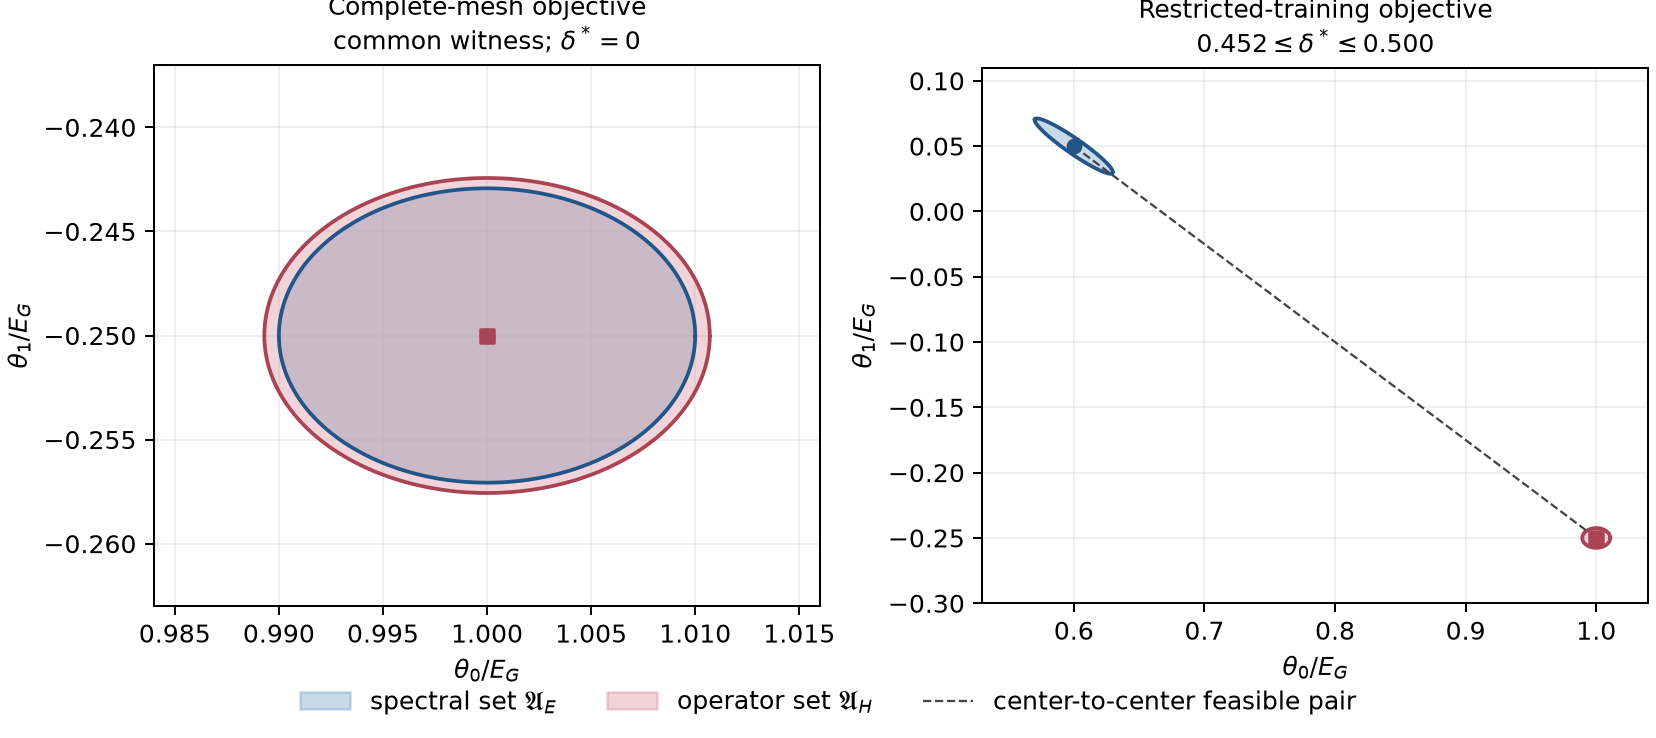
\includegraphics[width=.9\linewidth]{../../../../../calculations/ICMSEP2026/conference/paper_1/admissible-sets.png}\caption{Direct analytic admissible sets from the retained calculation. Complete-mesh objective construction admits a common witness; restricted objective construction produces certified positive separation. The figure depicts the fixed synthetic test settings, not material data.}\label{fig:analytic}\end{figure}

\subsection{Rank-two class under a finite alignment family (M3)}
The multiband test starts from the transported rank-two Hamiltonian $H(k)$ obtained from the four-state parent described in Supplement~\ref{supp:m2}. Write $\bar E(k)=\tfrac12\Tr H(k)$ and define
\begin{equation}\label{eq:m3}
H_{s,\lambda}(k)=\bar E(k)I+sE_GI+\lambda\big[H(k)-\bar E(k)I\big],\quad
-0.25\le s\le0.25,\quad0.4\le\lambda\le1.2.
\end{equation}
The parameter $s$ translates both retained bands, whereas $\lambda$ scales their splitting. The reference is $(s,\lambda)=(0,1)$. The alignment family is restricted to nine \emph{constant real} rotations with angles in $[-1.2,1.2]$ radians; it excludes arbitrary $k$-dependent recovery. This is an expressivity test for a specific finite union of admissible alignments.

For a normalized RMS spectral threshold $\tau_S=0.03$ and operator threshold $\tau_O=0.33$, $(0,1)$ is an exact common model within numerical reconstruction tolerance: its spectral loss is $7.59\times10^{-16}$ and its best accepted operator score is $0.3286318914$. Hence $\delta^*=0$. Tightening only the operator threshold to $0.31$ produces, in the frozen box, spectral feasibility only for $\lambda\gtrsim0.9354687052$ and operator feasibility only for $\lambda\lesssim0.8360013041$. Analytic quadratic reduction gives matching lower and constructive upper bounds,
\begin{equation}\label{eq:m3cert}
\boxed{\delta^*=0.0994674010>0.05,}
\end{equation}
where $0.05$ was the declared separation resolution. The 257 staggered withheld points are diagnostic only and do not determine thresholds or change accepted sets.

The thresholds were designed from the synthetic objective-construction-loss geometry to create two test regimes, then frozen before confirmatory evaluation; they were not selected blindly. The evidence establishes a correct bounded decision with a nonidentity finite alignment family, not a discovered material-dependent acceptance threshold or a general gauge-optimization result. The post-hoc threshold sweep places the onset of operator feasibility near $0.307420$, the $0.05$ resolution boundary near $0.313791$, the exact compatibility transition near $0.319264$, and admission of the original point at $0.328632$.

\begin{figure}[htbp]\centering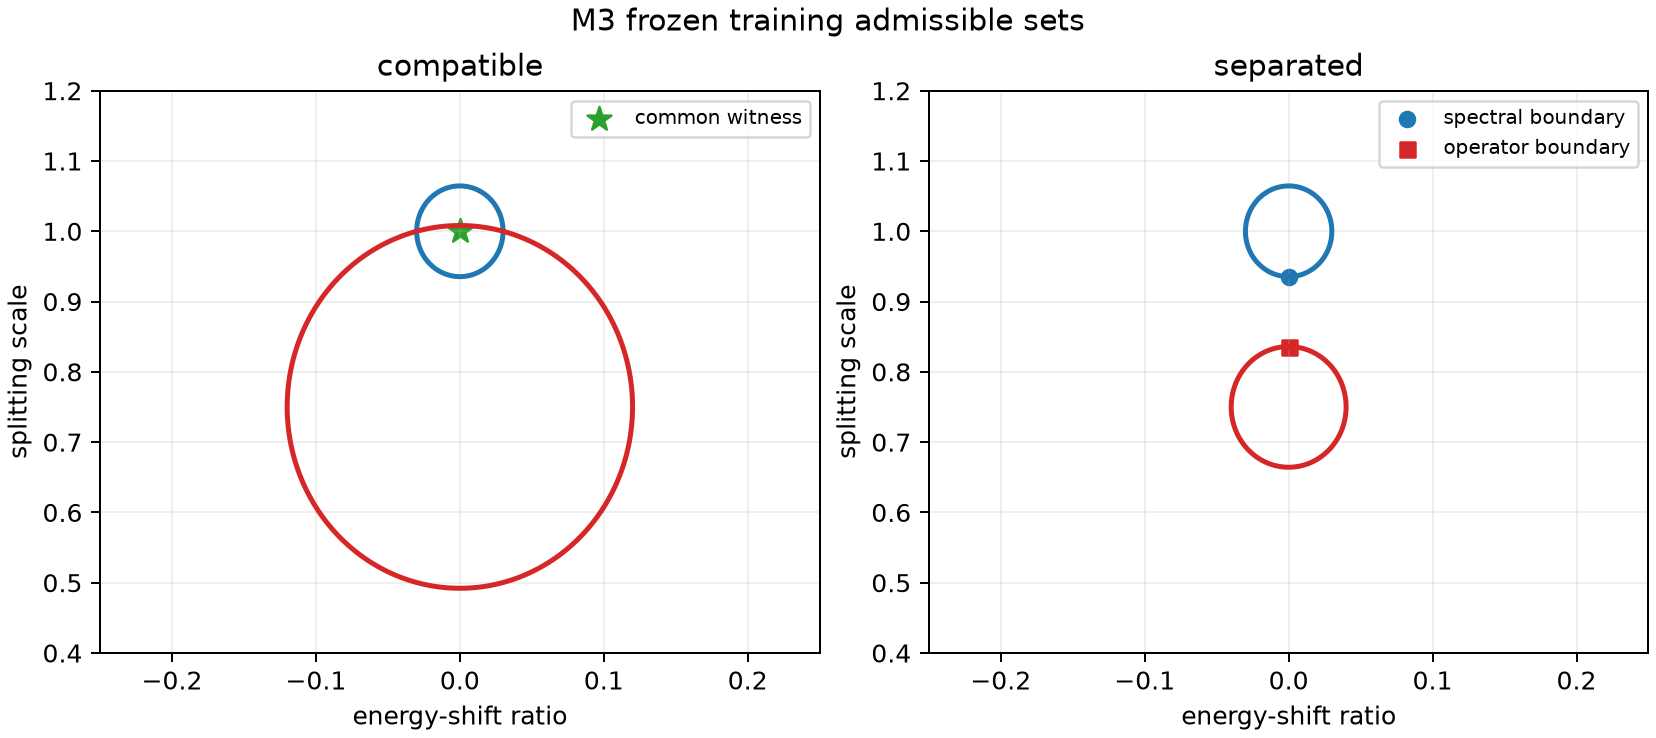
\includegraphics[width=.9\linewidth]{../../../../../calculations/ICMSEP2026/conference/paper_1/constrained-admissible-sets/constrained-admissible-sets-summary.png}\caption{M3 finite constrained-alignment admissible sets. The compatible case retains the reference witness; the tightened operator threshold yields certified separation in $(s,\lambda)$ coordinates.}\label{fig:m3}\end{figure}

\subsection{What the two certifications establish}
The scalar example isolates the role of the spectral objective-construction domain in a two-parameter finite-range class. M3 introduces a nontrivial retained subspace and a finite, nonidentity alignment restriction. Both decide feasibility for a \emph{fixed class and problem definition}; neither measures the minimum expressive class over a systematic hierarchy. In particular, decreasing $\tau_O$ can change compatibility even without changing the Hamiltonian basis or its number of parameters. A broader study of structural expressivity across Slater--Koster or hopping-shell classes remains a separate application, not an outcome demonstrated here.

\section{Supporting numerical evidence: transformation, truncation, and gauge}
\subsection{One-dimensional reconstruction and route equivalence (M1)}
The dimensionless parent is $\widehat H_{1\mathrm D}=-\dd^2/\dd x^2+0.5\cos x$ with period $a=2\pi$ and $E_G=1$. Plane-wave calculations were compared with the declared cutoff-$15$ \emph{finite represented} reference. For the lowest three checked eigenvalues, cutoff $P=5$ differs by at most $5.31\times10^{-13}E_G$, and an independently assembled finite-difference channel falls from $1.753\times10^{-2}E_G$ on 31 points to $2.598\times10^{-4}E_G$ on 255. The frozen M1 protocol did not record an isolation-gap result; the historical name ``isolated band'' is not independent evidence of isolation.

The complete 64-point transform of the lowest band reconstructs its sampled values within $4.17\times10^{-17}E_G$. Withheld maximum errors decline from $4.62\times10^{-2}E_G$ for an onsite model to $9.47\times10^{-9}E_G$ at $8a$. Equal-weight direct least squares and Fourier-mediated truncation in the \emph{same} complete Fourier model class agree in their coefficients within $7.38\times10^{-17}E_G$. This is an algebraic control under matched objectives, not a claim that general reduction routes commute. See Supplement~\ref{supp:m1} for the complete sequences.
\begin{figure}[htbp]\centering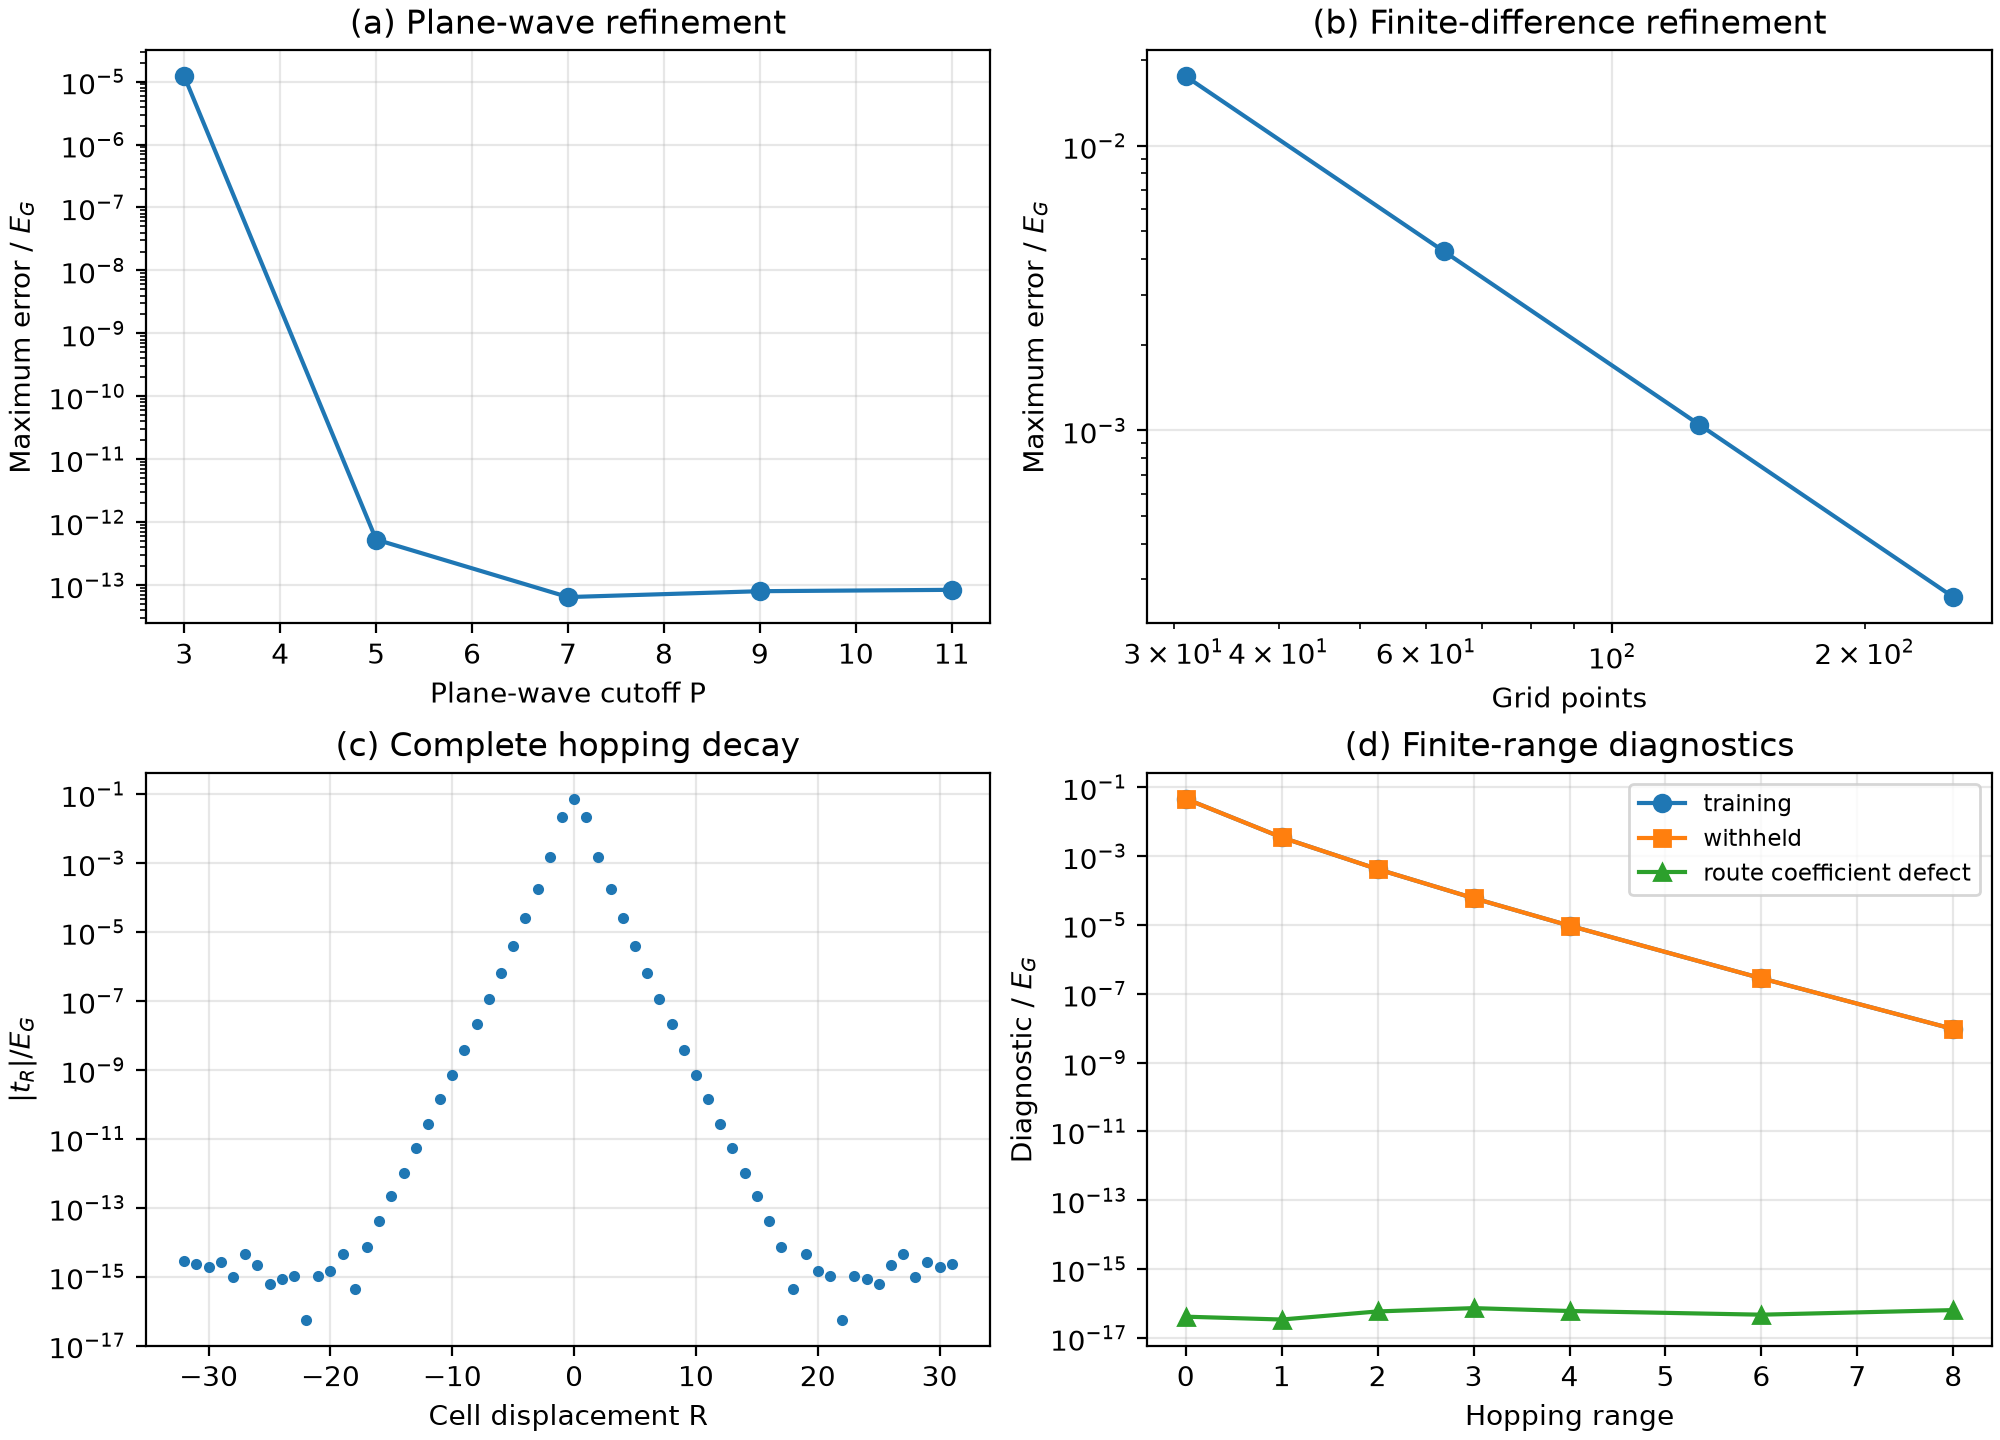
\includegraphics[width=.95\linewidth]{../../../../../calculations/ICMSEP2026/conference/paper_1/isolated-band/isolated-band-summary.png}\caption{M1 parent refinement, hopping decay, and objective-construction/withheld finite-range errors. Complete discrete reconstruction and finite-range approximation are evaluated separately.}\label{fig:m1}\end{figure}

\subsection{Rank-two gauge attack and finite-range locality (M2)}
M2 uses a gapped four-state block polynomial $H_4(k)=T_0+e^{2\pi ik}T_1+e^{-2\pi ik}T_1^\dagger$ and retains its lowest two eigenstates. The observed external gap is $1.056646\ldots$ and the minimum neighboring/closure overlap singular value is $0.9999829$. The smooth periodic internal attack $A(k)$ rotates the retained frame while preserving its projector within $3.24\times10^{-16}$ and its spectrum. Its attacked-frame operator matrices differ by up to $0.9972$ in Frobenius norm.

Pointwise Procrustes recovery of the known inverse attack reduces the matrix defect to $9.83\times10^{-16}$; a separate family allowing only one global unitary leaves a maximum residual $0.7443$. The attack redistributes Fourier block coefficients: writing $H(k)=\sum_R e^{2\pi ikR}T_R$ and $A(k)=\sum_m e^{2\pi ikm}A_m$ gives $\widetilde T_Q=\sum_{m,n}A_m^\dagger T_{Q+m-n}A_n$. At range eight, the attacked omitted-block norm is $5.65\times10^{-5}$ and withheld maximum spectral error is $7.04\times10^{-5}$; the recovered representation gives approximately $1.6\times10^{-14}$ and $1.2\times10^{-14}$. Thus gauge-equivalent spectral information need not be equally compressible in a prescribed short-range class.
\begin{figure}[htbp]\centering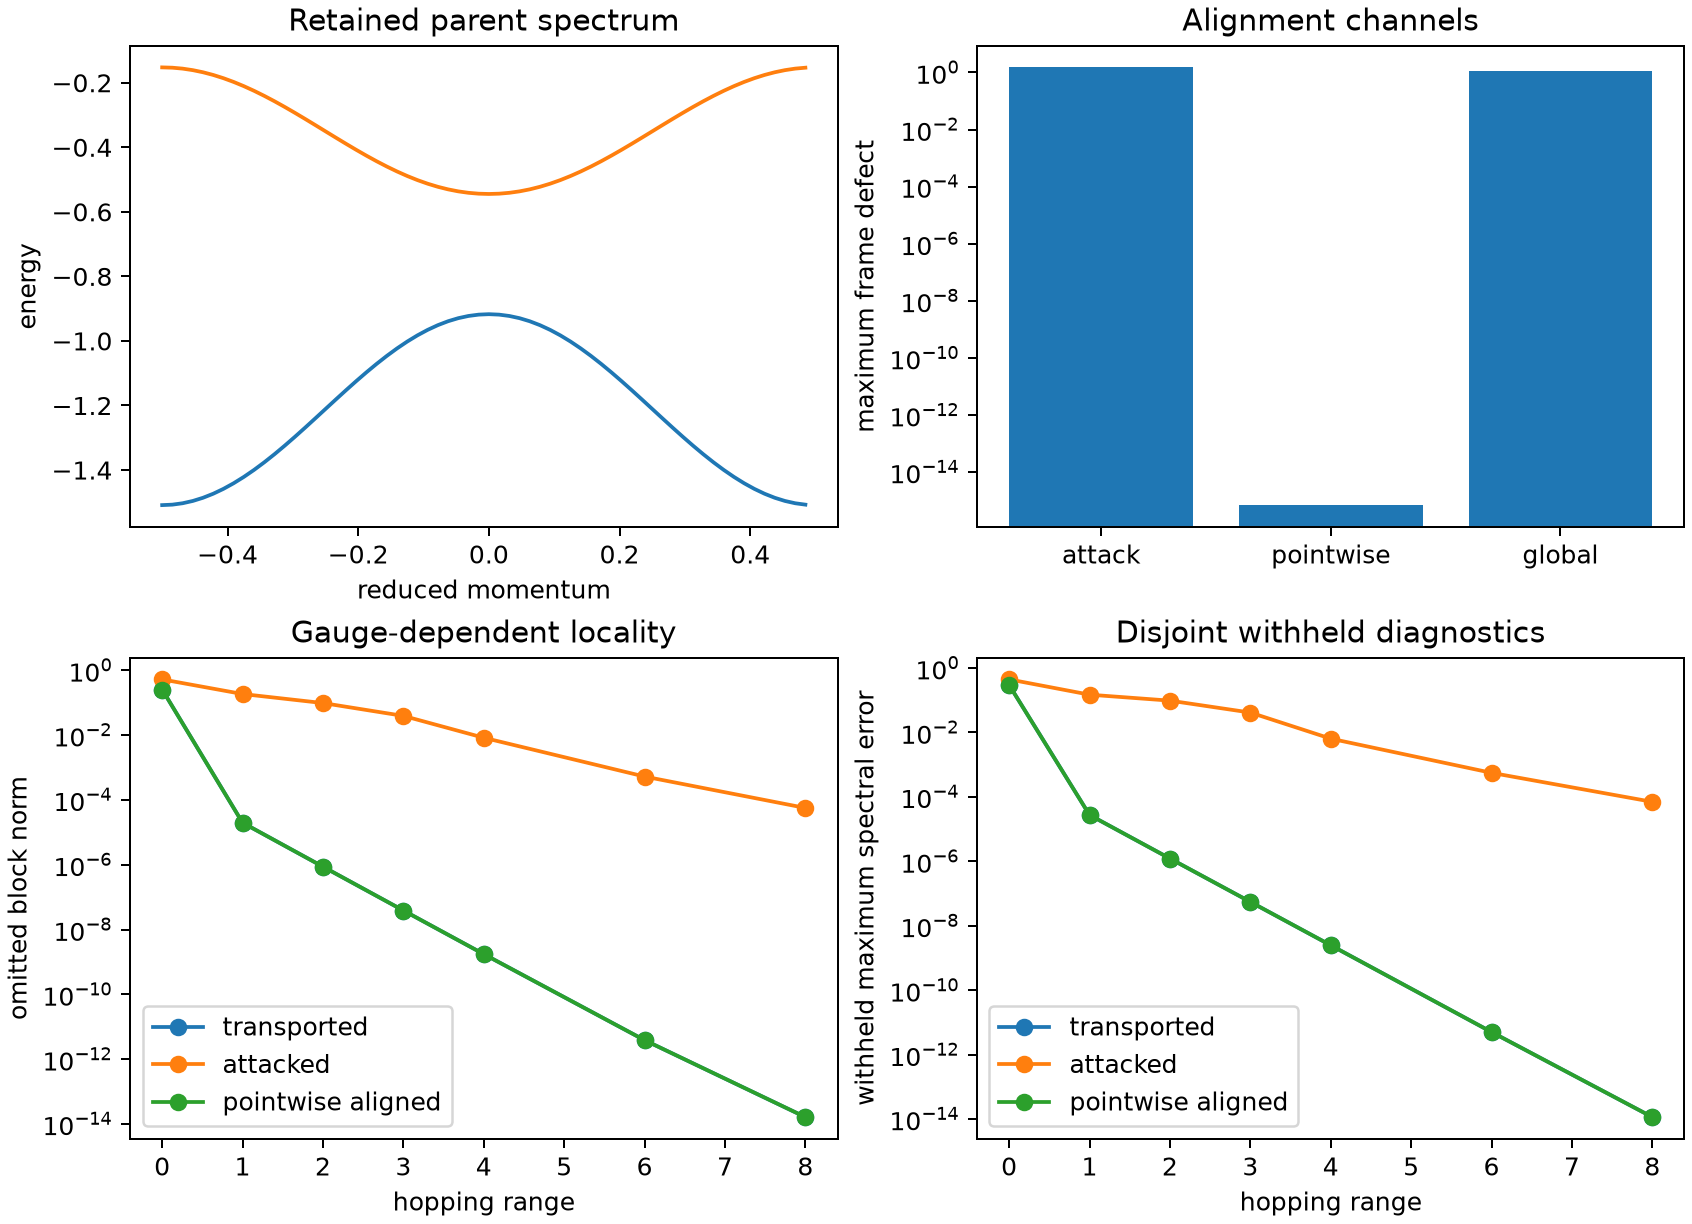
\includegraphics[width=.95\linewidth]{../../../../../calculations/ICMSEP2026/conference/paper_1/multiband-alignment/multiband-alignment-summary.png}\caption{M2 retained spectrum, pointwise versus global alignment, omitted hopping norms, and disjoint withheld errors.}\label{fig:m2}\end{figure}

\subsection{Two-dimensional coupling, shells, and composite-frame locality}
The second synthetic parent is
\begin{equation}\label{eq:2d}
\widehat H_{2\mathrm D}=-\nabla^2+0.5\cos x+0.5\cos y+\lambda_{xy}\cos x\cos y.
\end{equation}
At $\lambda_{xy}=0$ the represented Kronecker-sum defect is zero and the product-spectrum defect is $3.55\times10^{-14}E_G$. Increasing $\lambda_{xy}$ to $0.30$ raises the mixed-direction hopping norm from a $3.00\times10^{-15}E_G$ floor to $1.94\times10^{-3}E_G$. At the strongest coupling, withheld RMS interpolation errors fall from $5.75\times10^{-2}E_G$ for the onsite shell to $1.70\times10^{-6}E_G$ for the complete finite transform. The latter reproduces its own $15\times15$ mesh within $1.11\times10^{-15}E_G$ but retains nonzero error on the independent $31\times31$ mesh, separating exact sampled reconstruction from unsampled interpolation.

A smooth projected frame and periodic rough internal gauge for the lowest three bands agree spectrally within $1.22\times10^{-15}E_G$ and in unordered discrete Wilson-loop eigenphases within $2.22\times10^{-15}$. The finite-mesh Chern winding diagnostic is zero in both. Nevertheless the finite-supercell spread changes from $24.90a^2$ to $67.70a^2$, and the omitted hopping norm beyond squared-radius shell 18 from $1.38\times10^{-2}E_G$ to $5.25\times10^{-1}E_G$. These are finite-mesh localization and representational-compressibility diagnostics, not a continuum topological classification \cite{resta1994,zak1989,thouless1982,niu1985}.
\begin{figure}[htbp]\centering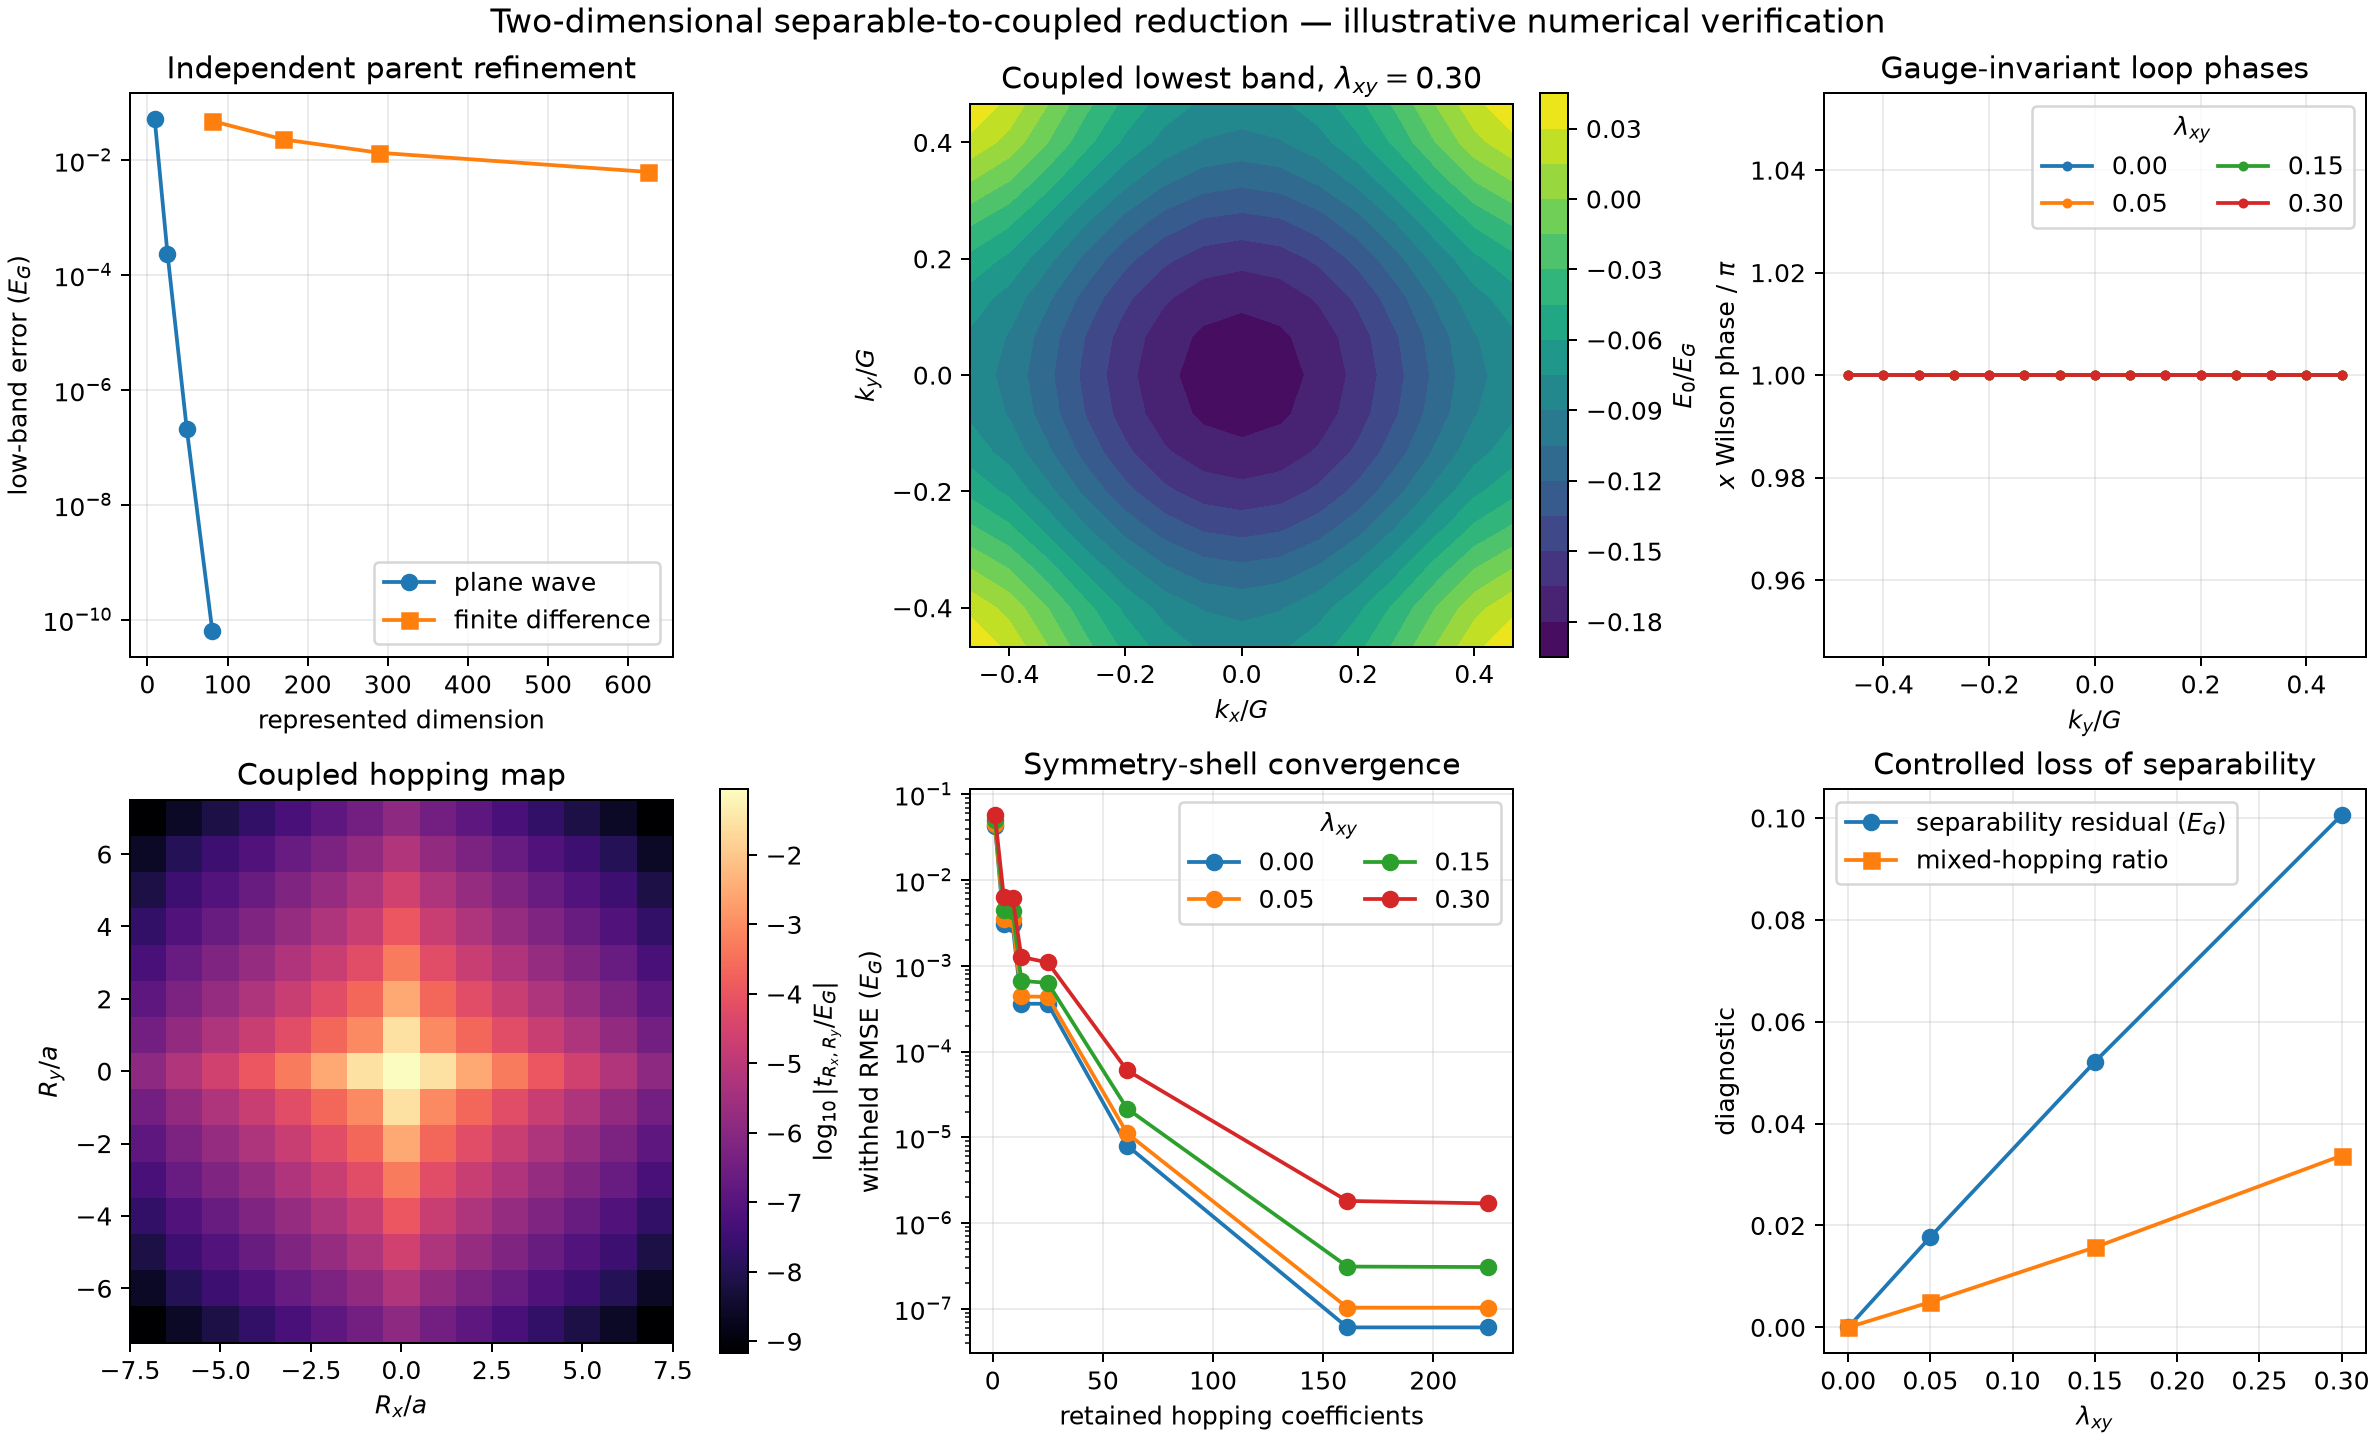
\includegraphics[width=.96\linewidth]{../../../../../calculations/research-monograph/periodic-2d/summary.png}\caption{Two-dimensional parent and coupling controls, hopping shells, and withheld spectral convergence.}\label{fig:2d}\end{figure}
\begin{figure}[htbp]\centering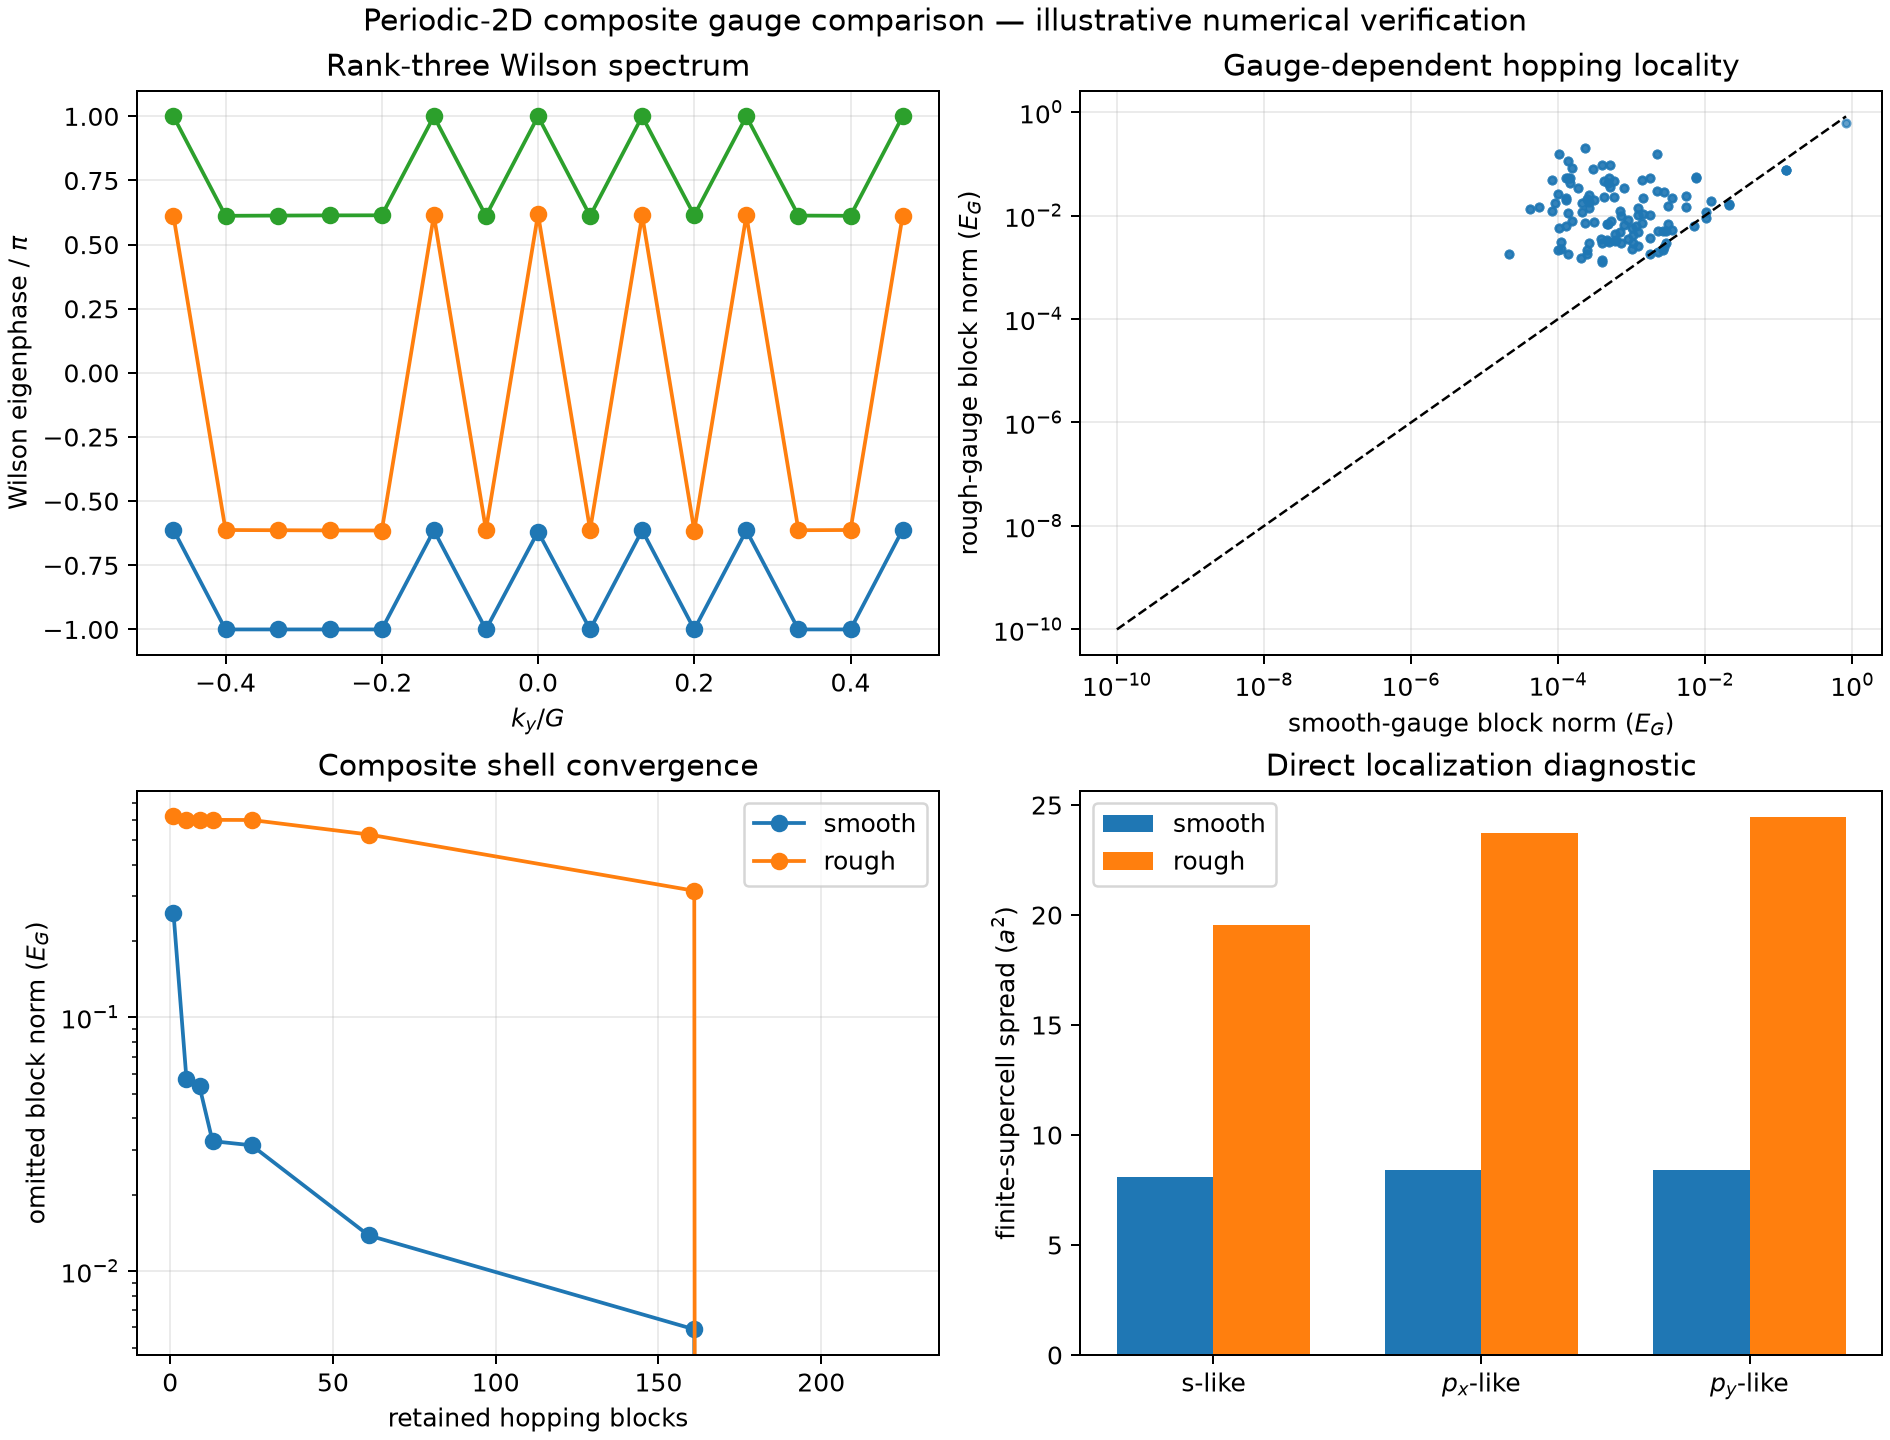
\includegraphics[width=.96\linewidth]{../../../../../calculations/research-monograph/periodic-2d/composite-summary.png}\caption{Composite-frame gauge-locality control: invariant subspace/spectral diagnostics coexist with different finite-supercell localization and hopping tails.}\label{fig:gauge}\end{figure}

\subsection{Wannier90-selected gauge: a finite bridge}
A separately retained synthetic two-dimensional calculation used Wannier90~3.1.0 on a $15\times15\times1$ mesh with three trial projections and no disentanglement. The direct projected frame and selected Wannier90 frame have maximum projector defect $2.65\times10^{-10}$; pointwise identification reduces represented-operator discrepancy to $3.57\times10^{-10}E_G$. A bounded search over integer orbital translations in $[-1,1]^2$ followed by a single constant orbital unitary instead leaves an operator defect $1.490E_G$. In the common finite-supercell spread estimator, the Wannier90 and direct values are $6.1359a^2$ and $24.5163a^2$; at squared-radius 50 the omitted hopping norms are $2.72\times10^{-4}E_G$ and $5.90\times10^{-3}E_G$.

This is useful algorithm-selected evidence of the same locality mechanism. It is \emph{not} a first-principles material calculation; the external execution was retained historically, not rerun for this manuscript. A six-case sensitivity study is nonmonotone and reaches different localization basins, preventing claims of mesh-, cutoff-, or basin-independent localization (Supplement~\ref{supp:wannier}).

\subsection{Tutorial-scale silicon: same-frame operator decomposition and a negative truncation result}\label{sec:silicon}
To test whether the represented-operator machinery can be applied to material-generated data without silently declaring a production-level Hamiltonian, we retain a read-only preview of the official Wannier90~3.1.0 \texttt{examples/example11} silicon tutorial. Post-hoc byte-identity checks match four original input files to that upstream tutorial. The executed \texttt{silicon.win} changes no numerical setting; it adds only \texttt{write\_hr=true} and \texttt{write\_u\_matrices=true} to request additional output artifacts. The retained QE~7.5--Wannier90~3.1.0 source run uses a legacy ultrasoft PBE pseudopotential, a 25-Ry wavefunction cutoff, 12 parent bands, four retained Wannier functions, and a $4\times4\times4$ Wannier mesh. None of these tutorial settings is claimed to be a converged silicon calculation.

At each of the 64 reciprocal samples, the source analysis forms $W(\bm k)=U_{\rm dis}(\bm k)U(\bm k)$ and constructs, in the \emph{same} rank-four frame,
\begin{align}\label{eq:silicon}
 H^W(\bm k)&=W^\dagger(\bm k)\,\operatorname{diag}(\epsilon)\,W(\bm k),\\
 T^W(\bm k)&=W^\dagger(\bm k)C_{\rm PW}^\dagger(\bm k)\,\operatorname{diag}\!\left(\frac{|\bm k+\bm G|^2}{2}\right) C_{\rm PW}(\bm k)W(\bm k),\\
 R^W(\bm k)&=H^W(\bm k)-T^W(\bm k).
\end{align}
Here $C_{\rm PW}$ is the matrix of plane-wave pseudo-wavefunction coefficients and $\epsilon$ denotes the parent eigenvalues included in the retained projection. The finite represented remainder $R^W$ must \emph{not} be identified with a continuous local scalar potential: the ultrasoft pseudopotential and finite representation prevent that inference. The same-frame identity holds with a maximum defect of $1.52\times10^{-15}$~eV. An independent route from the native \texttt{\_hr.dat} file differs by $1.28\times10^{-5}$~eV in maximum Frobenius norm.

The shell-resolved block norms in Fig.~\ref{fig:silicon-components} make the component contrast visible. At every nonzero canonical radius on this finite mesh, the maximum $\|T^W(\bm R)\|_F$ exceeds the maximum $\|R^W(\bm R)\|_F$, by factors from approximately $1.24$ to $2.67$. At many shells, $\|H^W(\bm R)\|_F$ is smaller than either component, reflecting cancellation in the exact relation $H^W=T^W+R^W$. The curves are nonmonotone and contain only 64 canonical representatives, so they do not establish asymptotic decay exponents or prove that the kinetic component decays more slowly on the infinite lattice.
\begin{figure}[htbp]\centering
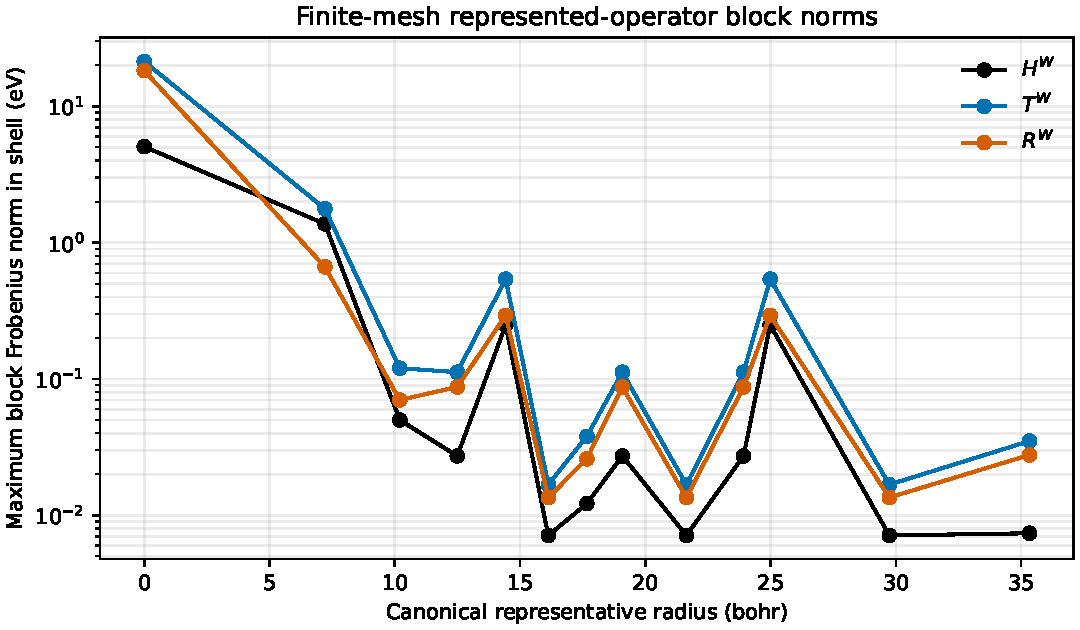
\includegraphics[width=.91\linewidth]{../../../../../calculations/ICMSEP2026/conference/paper_1/silicon-wannier-kinetic-preview/real-space-shell-block-norms.pdf}
\caption{Component-resolved finite-mesh block norms for the official Wannier90~3.1.0 silicon tutorial representation. Each point is the maximum Frobenius norm among blocks at one canonical representative radius. The kinetic blocks exceed the non-kinetic-remainder blocks at every nonzero sampled radius, while the nonmonotone finite-mesh curves do not determine an infinite-lattice decay rate. The represented remainder $R^W$ is not an identified continuous scalar potential.}\label{fig:silicon-components}
\end{figure}

A complete inverse finite transform contains 64 centered lattice blocks. Retaining 57 blocks still leaves maximum ordered-eigenvalue errors of $0.0207$~eV for $H^W$, $0.0843$~eV for $T^W$, and $0.0636$~eV for $R^W$. All 64 blocks recover their sampled matrices to roundoff. Thus successful total-Hamiltonian interpolation or complete-mesh reconstruction cannot be taken as evidence that the separate components admit the same aggressive short-range approximation. These errors establish failure of \emph{the tested truncation}, not the infeasibility of every compact silicon Hamiltonian class: no thresholded admissible-set map or global incompatibility certificate is constructed for silicon.
\begin{figure}[htbp]\centering
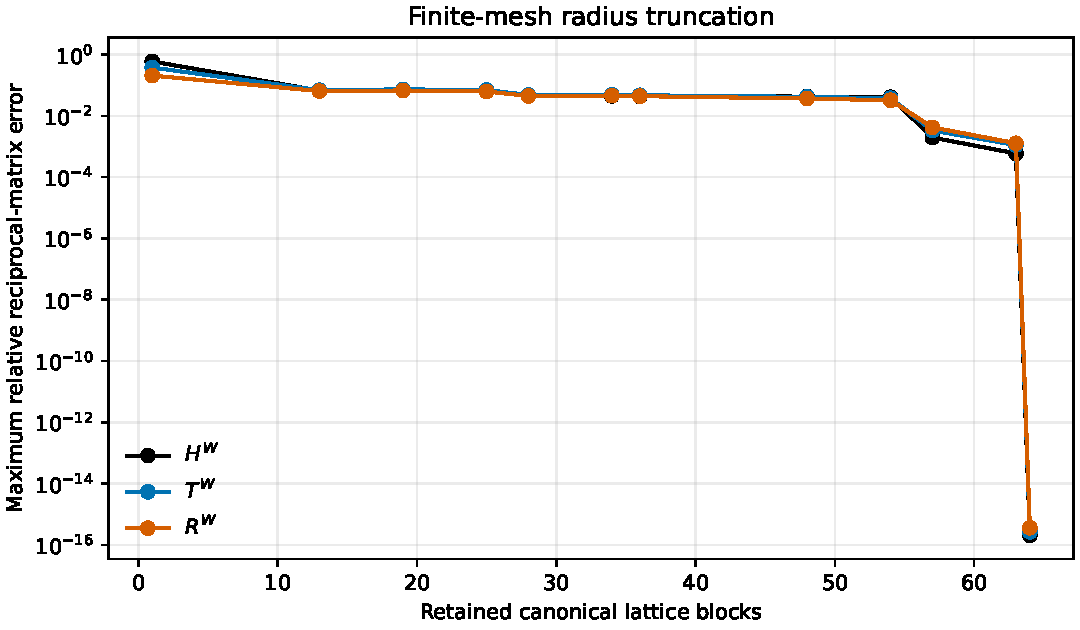
\includegraphics[width=.91\linewidth]{../../../../../calculations/ICMSEP2026/conference/paper_1/silicon-wannier-kinetic-preview/real-space-truncation-relative-error.pdf}
\caption{Negative finite-mesh truncation result from the official Wannier90~3.1.0 silicon tutorial setting, reproduced from the supplied source manuscript. Relative reciprocal-matrix errors apply to its $4\times4\times4$ representation. The final drop at 64 blocks reflects complete discrete reconstruction, not infinite-lattice decay or continuum convergence.}\label{fig:silicon}
\end{figure}
The preview is a material-derived software and numerical feasibility check, not validated silicon physics. It does not establish reciprocal-mesh or plane-wave convergence, a physically adequate short-range kinetic model, reliable silicon effective masses, or authenticated causal provenance of all source-run outputs. The identity of the input bytes is confirmed post hoc, but a pre-existing authenticated production-lineage manifest was unavailable. Supplement~\ref{supp:silicon} records the scope and data boundary.

\section{Interpretation, evidence boundaries, and implications}
Three logically distinct conclusions emerge. First, a reduction model class has an operational expressivity meaning only relative to specified information requirements: a spectral target and an aligned operator target. Second, the compatibility disposition can be established constructively or through genuine lower-bounding arguments, not by an optimizer's failure. Third, nontrivial gauge structure and hopping truncation explain why the spectral and operator constraints are not redundant for localized Hamiltonians.

Restricting a periodic Hamiltonian to a finite-dimensional or finite-range model class can introduce competing demands between spectral fidelity and real-space operator locality. When fitting reduced parameters, residual discrepancies may be absorbed into insufficiently constrained degrees of freedom, including unrestricted gauge rotations or hopping terms that violate the intended orbital and locality structure. A low spectral residual can then conceal poor operator fidelity or a loss of real-space compressibility. The coequal spectral and operator admissible-set formulation makes spectral and aligned-operator requirements explicit, while localization requires a separate tail or structural constraint: a common feasible witness establishes that the declared model class can satisfy both, whereas certified positive separation $\delta^*>0$ establishes incompatibility under the fixed alignment family, losses, and tolerances. This distinguishes insufficient model expressivity from optimization failure without attributing physical significance to arbitrary representation artifacts.

The controlled calculations are not interchangeable evidence. M1 checks exact finite transforms and matched reduction routes; M2 checks rank-two gauge alignment and compressibility; the two-dimensional examples show mixed-direction hopping and composite-frame localization; the Wannier90 bridge tests one algorithm-selected frame; the silicon tutorial preview tests same-frame projection and exposes the failure of a particular aggressive componentwise truncation; the direct and M3 cases alone instantiate thresholded admissible-set decisions. No general global optimization method for arbitrary $k$-dependent gauges is demonstrated. The silicon tutorial uses first-principles-generated input artifacts but does not validate a converged Si, Si:P, or Si:B Hamiltonian or establish any silicon admissible-set separation.

\begin{table}[htbp]\centering\small
\caption{Claims established by the retained controlled evidence.}\label{tab:scope}
\begin{tabular}{p{.20\linewidth}p{.36\linewidth}p{.35\linewidth}}\toprule
Component & Established within fixed specification & Not established\\\midrule
Direct scalar class & Exact common witness and positive rational separation enclosure & General finite-range-class impossibility\\
M3 rank-two class & Common witness and exact certified gap under nine constant rotations & Incompatibility under arbitrary smooth gauges\\
M1 & Complete discrete reconstruction and matched-route agreement & Universal hopping cutoff or continuum control\\
M2 & Gauge-dependent short-range compressibility, distinct alignment channels & General alignment optimizer\\
2D cases & Mixed hoppings, shell hierarchy, gauge-locality differences & Material-specific locality or topological theorem\\
Wannier90 bridge & Finite algorithm-selected localization comparison & First-principles validation or global MLWF optimality\\
Silicon tutorial preview & Same-frame rank-four decomposition; substantial finite-mesh component truncation errors & Production convergence, material adequacy, certified silicon expressivity\\\bottomrule
\end{tabular}
\end{table}

A natural next application is a sequence of structurally restricted Hamiltonian classes with fixed data and tolerances---for example, increasingly expressive orbital-block and neighbor-shell models. That comparison would identify which restrictions prevent simultaneous spectral and operator adequacy. It remains future work. The present contribution is the bounded feasibility-and-certification formulation, supported by controlled examples with explicit evidence limitations.

\section{Conclusions}
Model-class expressivity in periodic Hamiltonian reduction can be formulated as the existence of a common Hamiltonian satisfying both spectral and aligned-operator requirements. The existence of an explicit common witness proves compatibility. When both admissible sets are nonempty, positive certified separation proves incompatibility; numerical failure to locate an intersection remains inconclusive. The analytic nearest-neighbor example and constrained rank-two example demonstrate both decisions under deliberately specified synthetic test settings. Independent one- and two-dimensional tests establish the numerical distinction between transformation and truncation and show why gauge-equivalent bands can yield differently compressible localized Hamiltonians. The silicon tutorial preview adds a negative finite-mesh component-truncation observation without asserting a silicon compatibility decision. The paper supplies a controlled methodology for expressivity decisions, not a general infeasibility solver or a validated material model.

\section*{Acknowledgments}
\emph{Author to complete before submission.}
\section*{Data and code availability}
{\sloppy
Controlled input protocols, result records, independent reconstruction verifiers, figure sources, and checksum manifests are maintained in the project repository under \path{calculations/ICMSEP2026/conference/paper_1/} and \path{calculations/research-monograph/periodic-2d/}. A further bounded publication extraction is retained in the conference-paper \texttt{silicon-wannier-kinetic-preview/} subdirectory. It is not a complete production package. These working records are not presently represented as a public archival DOI. A release identifier, exact source revision, and authorization for any public deposit must be supplied before journal submission.
\par}

\clearpage\appendix
\section{Supplementary methods and retained numerical controls}
The supplement preserves the auditable protocol boundaries and detailed numerical data of the supplied manuscript. The main text gives the decisive analytical definitions and results; the sections below document the finite calculations and their limits. These records should be associated with the exact source-revision and artifact manifests before release.

\subsection{Gauge-orbit invariance and state-space mismatch}\label{supp:orbit}
Let $V_{\rm ref}$ and $V_{\rm red}$ have equal retained rank $r$ and let $\U$ be a nonempty family of unitary identifications $C:V_{\rm red}\to V_{\rm ref}$. With frozen $\SH$, weights, and $Z_{\rm ref}>0$, Eq.~\eqref{eq:LH} defines a continuous scalar loss in a constant $C$. A nonempty closed subset of $U(r)$ is compact, so the infimum is a minimum. For any selected $C_0\in\U$, Eq.~\eqref{eq:orbit} is nonnegative by the infimum property.

Under independent frame changes $A$ and $B$, let $H'_{\rm ref}=AH_{\rm ref}A^\dagger$, $H'_{\rm red}=BH_{\rm red}B^\dagger$, and $C'=ACB^\dagger$. If $\U'=\{ACB^\dagger:C\in\U\}$, then unitary invariance of the Frobenius norm implies $L_H'(C',\theta)=L_H(C,\theta)$. The correspondence is a bijection; the orbit infimum and the frame excess agree. This is \emph{covariance under the specified admissible family}, not freedom to expand the physically admissible family after fitting. A different rank with an authorized projection requires a separate embedding-error channel. Without any admissible identification the operator difference is undefined, though common-ambient-space projector and invariant spectral diagnostics may remain meaningful.

\subsection{Spectral projection and finite-range support}\label{supp:projection-locality}
Suppose a parent is exactly finite range in a declared orbital basis,
\begin{equation}\label{eq:finite-range-parent}
H(\bm k)=\sum_{\bm R\in S_0}e^{i\bm k\cdot\bm R}T_{\bm R},
\qquad |S_0|<\infty.
\end{equation}
For a spectral projector $P(\bm k)$, the embedded projected operator has coefficients
\begin{equation}\label{eq:projected-hopping}
T^{(P)}_{\bm R}=\frac{1}{|\mathrm{BZ}|}\int_{\mathrm{BZ}}e^{-i\bm k\cdot\bm R}P(\bm k)H(\bm k)P(\bm k)\,\mathrm{d}\bm k.
\end{equation}
These coefficients need not vanish outside $S_0$. An explicit one-dimensional example is the two-orbital nearest-neighbor Hamiltonian
\begin{equation}\label{eq:projection-two-band}
H(k)=\begin{pmatrix}
\Delta&t(1+e^{-ik})\\
t(1+e^{ik})&-\Delta
\end{pmatrix},
\qquad t\in\mathbb R,\quad \Delta\ne0.
\end{equation}
It obeys $H(k)^2=d(k)^2I$, where
\begin{equation}\label{eq:projection-dispersion}
d(k)=\sqrt{\Delta^2+4t^2\cos^2(k/2)},
\qquad E_\pm(k)=\pm d(k).
\end{equation}
The lower-band projector and its embedded projected operator are
\begin{align}
P_-(k)&=\tfrac12\left[I-H(k)/d(k)\right],\\
H_-(k)&=P_-(k)H(k)P_-(k)
      =-d(k)P_-(k)
      =\tfrac12\left[H(k)-d(k)I\right].\label{eq:projection-counterexample}
\end{align}
For generic $t\ne0$, $d(k)$ is not a finite Fourier polynomial. Hence $H_-(k)$ generally has nonzero coefficients beyond the parent's nearest-neighbor range even though it retains the lower eigenpair exactly; the compressed rank-one scalar $-d(k)$ is likewise not a finite Fourier polynomial. Because $\Delta\ne0$ keeps the two bands separated, this failure of exact finite support is compatible with rapid, including exponential, decay. The displayed matrix coefficients refer to the original two-orbital embedding; represented hopping matrices in a composite retained space additionally depend on the chosen internal frame.

This example separates three operations: spectral projection $H\mapsto PHP$, hopping truncation $H(\bm R)\mapsto\mathbf1_{\bm R\in S}H(\bm R)$, and structural restriction $H\mapsto H_j(\theta)\in\M_j$. The first preserves selected eigenpairs, the second imposes a translation domain, and the third imposes a model form. None alone supplies a simultaneous spectral--operator admissibility decision.

\subsection{M1: frozen one-dimensional protocol}\label{supp:m1}
The parent $-\dd^2/\dd x^2+0.5\cos x$ uses $a=2\pi$, reduced momentum $k/G\in[-1/2,1/2)$, plane-wave cutoffs $3,5,7,9,11$, and finite represented cutoff $15$ as reference. The production cutoff is $11$; finite-difference grids are $31,63,127,255$. Five parent momenta $-1/2,-1/4,0,1/4,1/2$ check the lowest three ordered bands. The objective-construction Fourier mesh has 64 points, symmetric hopping ranges are $0,1,2,3,4,6,8$, and 257 staggered disjoint points provide withheld evaluation. Numerical-consistency and coordinate tolerances are $10^{-12}$ and $10^{-14}$.
\begin{table}[h]\centering\small\caption{M1 parent refinement relative to the finite cutoff-$15$ representation.}\begin{tabular}{rrrr}\toprule Plane-wave cutoff & Maximum discrepancy ($E_G$) & FD grid & Maximum discrepancy ($E_G$)\\\midrule
3&$1.2107868\times10^{-5}$&31&$1.7532742\times10^{-2}$\\5&$5.3113069\times10^{-13}$&63&$4.2534046\times10^{-3}$\\7&$6.4837025\times10^{-14}$&127&$1.0471637\times10^{-3}$\\9&$8.0380147\times10^{-14}$&255&$2.5977169\times10^{-4}$\\11&$8.4487972\times10^{-14}$&&\\\bottomrule\end{tabular}\end{table}

For the centered half-open mesh $k_j/G=-1/2+j/N$, discrete Fourier columns have the phase-weighted orthogonality relation $N^{-1}\sum_j e^{2\pi i(S-R)k_j/G}=(-1)^{S-R}\delta_{R,S\ ({\rm mod}\ N)}$. Hence matched direct equal-weight least squares and Fourier truncation recover equivalent finite coefficients.
\begin{table}[h]\centering\small\caption{M1 finite-range objective-construction and withheld errors, omitted norm, and direct/mediated coefficient defect (all in $E_G$).}\begin{tabular}{rrrrr}\toprule Range & Training max & Withheld max & Omitted norm & Route defect\\\midrule
0&$4.6235761\times10^{-2}$&$4.6235757\times10^{-2}$&$3.0304372\times10^{-2}$&$4.16\times10^{-17}$\\1&$3.4907261\times10^{-3}$&$3.4907249\times10^{-3}$&$2.1876793\times10^{-3}$&$3.44\times10^{-17}$\\2&$4.1809353\times10^{-4}$&$4.1809323\times10^{-4}$&$2.5574449\times10^{-4}$&$5.91\times10^{-17}$\\3&$6.0054873\times10^{-5}$&$6.0054797\times10^{-5}$&$3.6185635\times10^{-5}$&$7.38\times10^{-17}$\\4&$9.5136497\times10^{-6}$&$9.5136313\times10^{-6}$&$5.6738480\times10^{-6}$&$6.09\times10^{-17}$\\6&$2.8158444\times10^{-7}$&$2.8158339\times10^{-7}$&$1.6575039\times10^{-7}$&$4.76\times10^{-17}$\\8&$9.4653550\times10^{-9}$&$9.4652958\times10^{-9}$&$5.5272060\times10^{-9}$&$6.47\times10^{-17}$\\\bottomrule\end{tabular}\end{table}

The complete mesh reconstruction and modular Hermiticity defects are $4.1661\times10^{-17}E_G$ and $2.0907\times10^{-18}E_G$. Maximum route sampled difference is $1.5649\times10^{-16}E_G$ and maximum Parseval residual $6.9389\times10^{-18}E_G^2$. The retained standalone verifier independently constructs the finite protocol without importing its producer action; reconstructed spectral, hopping, and diagnostic defects are $0$, $4.78\times10^{-17}$, and $2.73\times10^{-14}$, respectively. It shares numerical-library and floating-point conventions with the producer; this is finite-protocol reconstruction, not an independent physical oracle.

\subsection{M2: gapped parent, transport, and known gauge attack}\label{supp:m2}
The four-state Hermitian parent is $H_4(k)=T_0+e^{2\pi ik}T_1+e^{-2\pi ik}T_1^\dagger$, with
\[
T_0=\begin{pmatrix}-1.20&0.06&0&0\\0.06&-0.35&0&0\\0&0&1.00&0.04\\0&0&0.04&1.75\end{pmatrix},\qquad
T_1=\begin{pmatrix}0.15&0&0&0\\0&-0.10&0&0\\0.12&0&0.05&0\\0&0.10&0&-0.04\end{pmatrix}.
\]
The lowest two eigenstates define the retained rank-two subspace. Sixty-four centered objective-construction momenta and 257 disjoint staggered evaluation points are frozen. Polar frame transport includes reciprocal closure sewing. The known periodic attack is the real rotation $A(k)=\left(\begin{smallmatrix}\cos\vartheta&-\sin\vartheta\\\sin\vartheta&\cos\vartheta\end{smallmatrix}\right)$ with $\vartheta(k)=0.30+0.65\sin(2\pi k)+0.30\sin(4\pi k)$. It leaves the projector invariant while changing the represented Hamiltonian and hopping range.

Let $F_{\rm ref}(k_j)$ and $F_{\rm att}(k_j)$ denote the transported reference and attacked frames. At each objective-construction point, form the cross-overlap
\begin{equation}\label{eq:m2-pointwise-procrustes}
M_j=F_{\rm att}(k_j)^\dagger F_{\rm ref}(k_j)=L_j\Sigma_jV_j^\dagger .
\end{equation}
Sch\"onemann established the corresponding real orthogonal least-squares problem \cite{schonemann1966}. For the complex unitary form, identify $A$ in Higham's notation with $F_{\rm ref}(k_j)$ and $B$ with $F_{\rm att}(k_j)$, so that $B^\dagger A=M_j$. Higham's equations (2.1)--(2.3) give the SVD construction of the unitary polar factor, and Theorem 2.2, specifically inequality (2.4), proves that this factor minimizes the Frobenius residual over all unitary matrices \cite{higham1986}. Section 6.1 of the same article identifies the real specialization as the orthogonal Procrustes problem. Accordingly, the pointwise transformation is $U_j=L_jV_j^\dagger$. It right-multiplies the attacked frame and minimizes $\|F_{\rm att}(k_j)U-F_{\rm ref}(k_j)\|_F$ over $U\in U(2)$. With this convention, the attacked represented Hamiltonian is carried into the aligned coordinates as $U_j^\dagger H_{\rm att}(k_j)U_j$. The distinct one-global-unitary channel instead forms
\begin{equation}\label{eq:m2-global-procrustes}
B=\sum_jF_{\rm att}(k_j)^\dagger F_{\rm ref}(k_j)=L_B\Sigma_BV_B^\dagger
\end{equation}
and uses $U_{\rm glob}=L_BV_B^\dagger$, which minimizes the sum of the squared frame residuals over a single $U\in U(2)$. Thus the pointwise and global calculations optimize different admissible alignment families rather than two numerical approximations to the same problem.

For the constructed attack, $M_j=A(k_j)^\dagger$ is unitary at every objective-construction point, and the frozen global aggregate is nonsingular. Higham's Theorem 1.1 therefore makes each relevant unitary polar factor unique \cite{higham1986}. Rank-deficient overlaps would leave an undetermined unitary action between null spaces and would require either explicit rejection or a declared deterministic completion; neither case is exercised or qualified here.

The pointwise inverse attack is recovered within $6.77\times10^{-16}$, with aligned-frame defect $7.00\times10^{-16}$. The best frozen one-global-unitary channel is the constant rotation $-0.30$ radians; frame and operator maxima remain $1.131$ and $0.7443$. Complete Fourier reconstruction errors are $6.76\times10^{-16}$ (transported), $1.14\times10^{-15}$ (attacked), and $6.77\times10^{-16}$ (pointwise aligned), with block-Hermiticity defect at most $4.50\times10^{-17}$.
\begin{table}[h]\centering\small\caption{M2 selected omitted block norms and withheld maximum spectral errors.}\begin{tabular}{rrrrrr}\toprule Range&Transported tail&Attacked tail&Transported err.&Attacked err.&Aligned err.\\\midrule
0&$2.54\times10^{-1}$&$5.23\times10^{-1}$&$2.98\times10^{-1}$&$4.45\times10^{-1}$&$2.98\times10^{-1}$\\1&$1.98\times10^{-5}$&$1.85\times10^{-1}$&$2.76\times10^{-5}$&$1.49\times10^{-1}$&$2.76\times10^{-5}$\\4&$1.75\times10^{-9}$&$8.28\times10^{-3}$&$2.49\times10^{-9}$&$6.43\times10^{-3}$&$2.49\times10^{-9}$\\8&$1.63\times10^{-14}$&$5.65\times10^{-5}$&$1.15\times10^{-14}$&$7.04\times10^{-5}$&$1.15\times10^{-14}$\\\bottomrule\end{tabular}\end{table}

The standalone verifier independently assembles the parent, eigenspaces, transport, attack, alignments, and truncations. Its maximum dimensionless and energy defects are $1.33\times10^{-15}$ and $7.43\times10^{-15}$, below the frozen $10^{-11}$ tolerance. The retained software record reports Python 3.14.6, NumPy 2.5.1, SciPy 1.18.0, Matplotlib 3.11.1, and \texttt{ksdft2effmass 0.1.0.dev0}; the dirty source snapshot is bound by a recorded SHA-256 source digest.

\subsection{Direct analytic quadratic details}
For Eq.~\eqref{eq:scalar}, the fixed operator comparison uses the five distinct real-space translations, with a single global normalization. Completing squares in each exactly derived quadratic yields the centers in the main text. The lower eigenvalue enclosure for the restricted spectral quadratic can be taken as $\lambda_{E,\min}>91/1200$; the operator quadratic admits a radius $11/1000$ under the same excess budget. Together with a valid spectral radius $37/1000$, the center separation $1/2$ yields $\delta^*\ge1/2-37/1000-11/1000=113/250$. The feasible center pair bounds the distance from above by $1/2$. Four reciprocal evaluation points were excluded from both spectral objective-construction choices and never used to revise thresholds or certificates.

\subsection{M3: threshold design, sensitivity, and verification}\label{supp:m3}
The M3 operator set is a finite union of the passing quadratic regions associated with nine frozen real rotation angles. The 64 objective-construction points define both quadratic loss surfaces, while 257 staggered points remain withheld. The selected controls are spectral RMS threshold $0.03$, compatible operator RMS threshold $0.33$, separated operator RMS threshold $0.31$, and parameter-separation resolution $0.05$. The operator threshold was explicitly designed after analysis of the synthetic objective-construction geometry; it was frozen before the retained confirmatory execution but was not blind.

At $\tau_O=0.33$, the witness $(s,\lambda)=(0,1)$ passes using the $0.3$-radian constant alignment. With $\tau_O=0.31$, the limiting spectral and operator $\lambda$ values are $0.9354687052$ and $0.8360013041$, respectively; their difference gives the exact finite-family certificate stated in Eq.~\eqref{eq:m3cert}. In a separate post-hoc threshold sweep at $\tau_S=0.03$, the operator set first becomes feasible near $0.307420$, the distance drops below resolution at $0.313791$, the accepted sets first intersect at $0.319264$, and the original parameter becomes admissible at $0.328632$.
\begin{figure}[htbp]\centering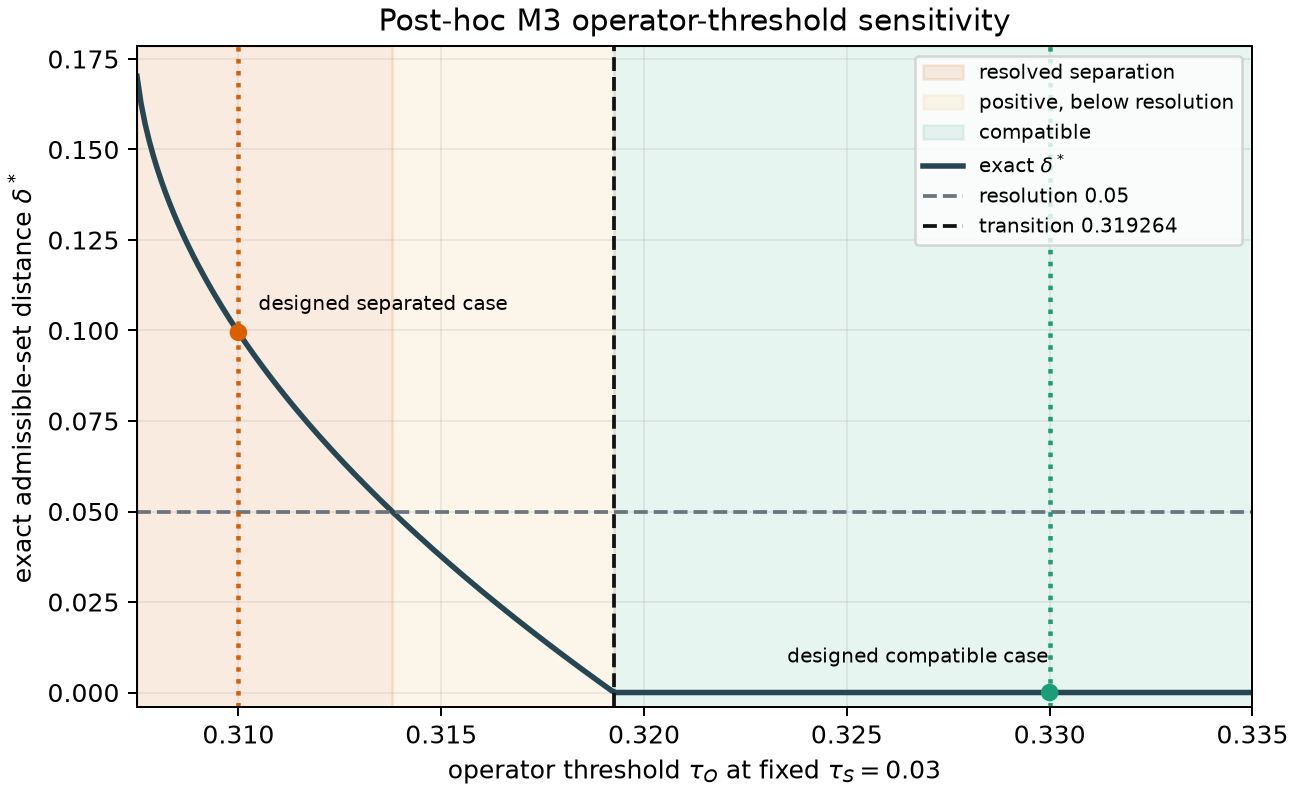
\includegraphics[width=.9\linewidth]{../../../../../calculations/ICMSEP2026/conference/paper_1/constrained-admissible-sets-threshold-sensitivity/operator-threshold-sensitivity.png}\caption{Post-hoc operator-threshold sensitivity for the retained M3 quadratic geometry. This is not an independently preregistered confirmatory sweep.}\end{figure}
The retained record includes nine amendments, including correction of a previous erroneous objective-construction/evaluation-coordinate diagnosis; the amendments are disclosed rather than presented as immutable preregistration. Independent library and standalone reconstruction defects are $1.33\times10^{-15}$ and $4.66\times10^{-15}$, both below the frozen $10^{-11}$ tolerance. The verifiers do not establish independent scientific validity or trusted chronology.

\subsection{Two-dimensional gauge and separability controls}
For Eq.~\eqref{eq:2d}, the $\lambda_{xy}=0$ Kronecker-sum control reconstructs the product spectrum within $3.55\times10^{-14}E_G$. A rank-two degenerate-cluster control preserves the projector under a Hadamard rotation while individual overlaps become $1/\sqrt2$. An anisotropic control gives principal masses $1.184m$ and $2.112m$ while retaining time reversal and two reflection symmetries within $3.60\times10^{-14}E_G$. The composite-gauge comparison uses discrete polar Wilson links on closed sewn loops. Equal Wilson eigenphase multisets and a zero finite-mesh winding are only gauge-consistency diagnostics, not an independently certified continuum Chern invariant.

\subsection{Wannier90 bridge: finite controls and sensitivity}\label{supp:wannier}
The synthetic parent is $-\nabla^2+0.5\cos x+0.5\cos y+0.15\cos x\cos y$, represented on a $15\times15\times1$ mesh with the lowest-three-band subspace, centered $s,p_x,p_y$ trial projections, no disentanglement, and Wannier90~3.1.0. The retained balanced execution met the $10^{-12}$ spread-change criterion at iteration 94. Native Wannier90 Berry-link spread and common finite-supercell spread are different estimators: the native balanced spread is $0.7094a^2$; the common-grid Wannier90 and direct projected spreads are $6.1359a^2$ and $24.5163a^2$. Native \texttt{\_hr.dat} mesh reconstruction has maximum matrix and spectral differences $3.06\times10^{-5}E_G$ and $2.23\times10^{-5}E_G$, retained as finite decimal serialization effects.
\begin{table}[h]\centering\small\caption{Six retained Wannier90 sensitivity cases. Changes are not a convergence sequence.}\begin{tabular}{lrr}\toprule Case&Native spread ($a^2$)&Radius-50 tail ($E_G$)\\\midrule
Reference $P=3$, $N=15$, $c=15$&0.7094&$2.72\times10^{-4}$\\Mesh $N=19$&1.7901&$4.52\times10^{-2}$\\Cutoff $P=2$&1.7072&$3.30\times10^{-2}$\\Cutoff $P=4$&1.7024&$3.38\times10^{-2}$\\Embedding $c=12$&0.7093&$2.72\times10^{-4}$\\Embedding $c=18$&1.7024&$3.38\times10^{-2}$\\\bottomrule\end{tabular}\end{table}
\begin{figure}[htbp]\centering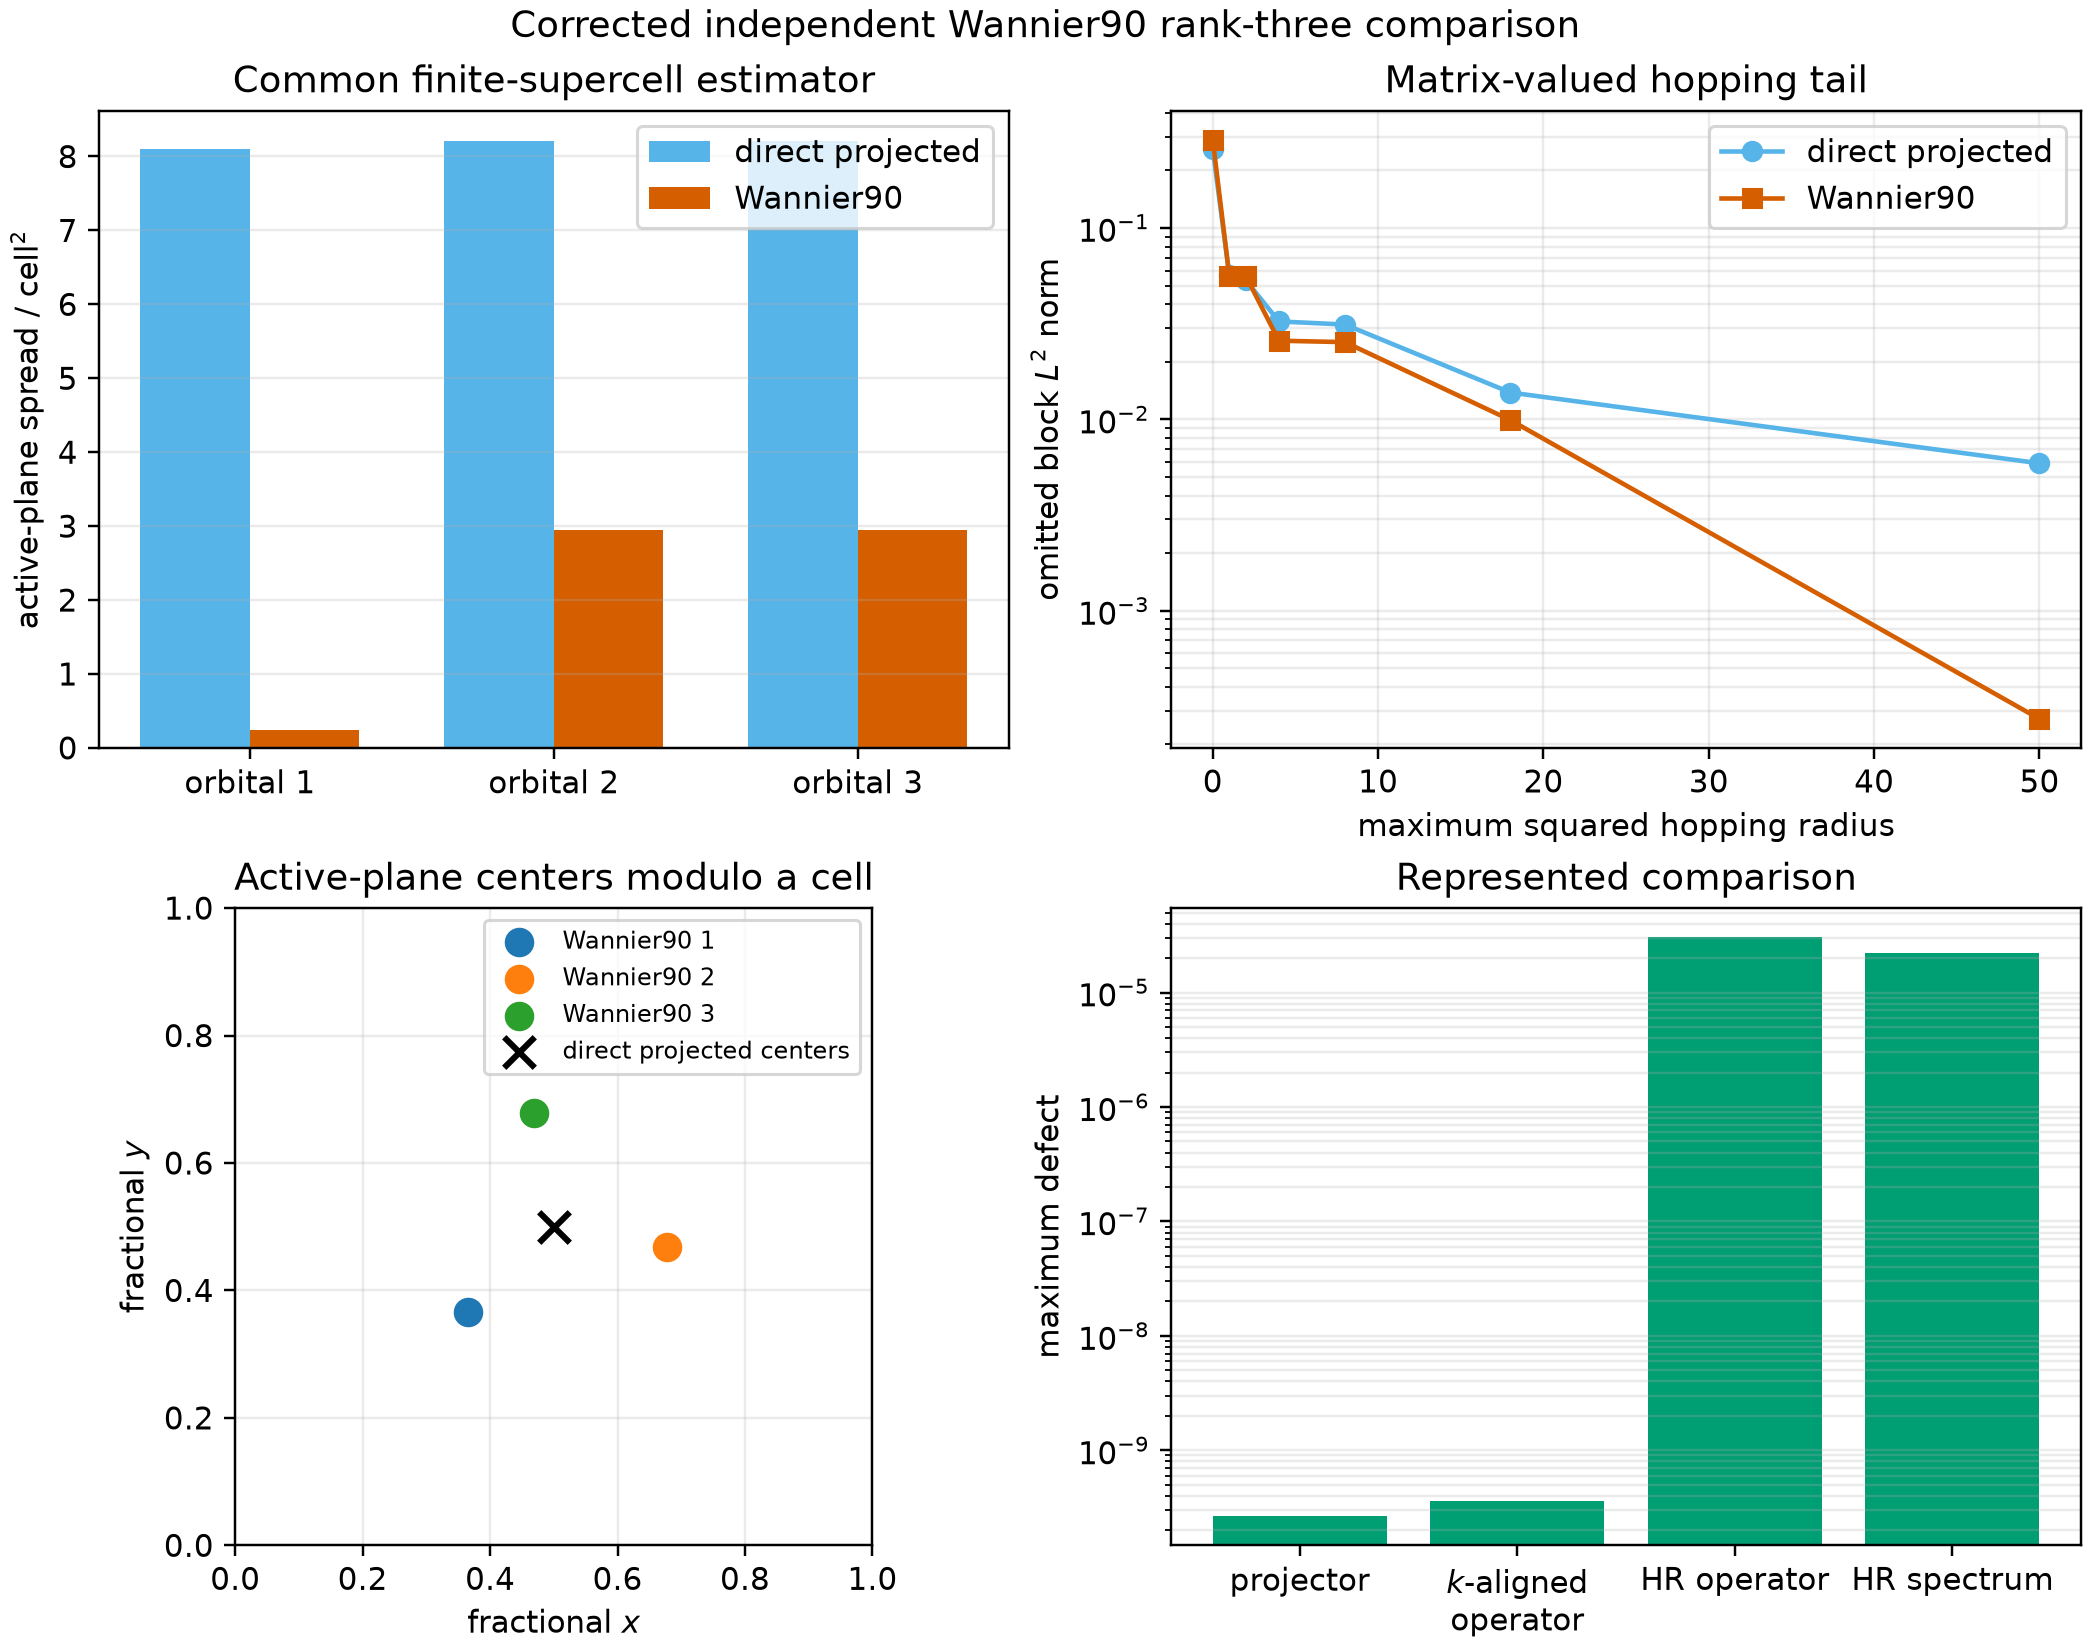
\includegraphics[width=.9\linewidth]{../../../../../calculations/research-monograph/periodic-2d/wannier90-balanced-summary.png}\caption{Retained finite Wannier90 comparison from the source manuscript. Native and common-estimator spreads are not interchangeable.}\end{figure}

\subsection{Silicon tutorial preview: numerical settings, negative result, and provenance}\label{supp:silicon}
This read-only calculation uses source bytes correlated to the four official Wannier90~3.1.0 \texttt{examples/example11} input files. The source-run \texttt{silicon.win} adds only two output requests (\texttt{write\_hr=true}, \texttt{write\_u\_matrices=true}) and leaves numerical settings unchanged. The upstream record uses QE~7.5, an ultrasoft PBE pseudopotential, 25~Ry, 12 parent bands, four Wannier orbitals, and a $4\times4\times4$ sampling mesh. The tutorial's smooth total-band plots are an interpolation illustration, not convergence data for the kinetic and remainder components.

The rank-four matrices in Eq.~\eqref{eq:silicon} are assembled in one common Wannier frame, with a same-frame subtraction defect of $1.52\times10^{-15}$~eV. The independent native \texttt{\_hr.dat} route gives a maximum Frobenius difference of $1.28\times10^{-5}$~eV. The 64-point finite inverse transform reconstructs the sampled matrices at machine precision. Table~\ref{tab:silicon} gives the tested truncation error at 57 of the 64 canonical blocks; it does not establish decay for the infinite lattice.
\begin{table}[htbp]\centering\small
\caption{Maximum ordered eigenvalue error for the finite-mesh silicon tutorial preview after retaining 57 of 64 centered lattice blocks.}\label{tab:silicon}
\begin{tabular}{lc}\toprule Component & Maximum error (eV)\\\midrule
Total represented Hamiltonian $H^W$ & 0.0207\\
Represented kinetic operator $T^W$ & 0.0843\\
Non-kinetic remainder $R^W$ & 0.0636\\\bottomrule\end{tabular}
\end{table}
The imported publication subset includes source JSON, figure inputs, upstream tutorial input correlation, external output manifest, and local checksums. Post-hoc SHA-256 correspondence of the input files does not certify the causal output lineage: the preview did not consume a pre-existing authenticated production-lineage manifest. No QE or Wannier90 run was repeated as part of the manuscript. No independent reciprocal-mesh, cutoff, projector-convergence, effective-mass, or symmetry-alignment acceptance study is reported. This is a negative \emph{particular-truncation} result rather than a proof of nonexpressivity for any general silicon model class.

\subsection{Evidence provenance and release boundary}
The original protocol/result packages are maintained in the project repository, principally in the conference paper 1 calculation directory (isolated-band, multiband-alignment, constrained-admissible-sets, and threshold-sensitivity subdirectories) and in the research-monograph periodic-2d directory. Each retained calculation is accompanied by protocol documents, result records, independently assembled finite verifiers, selected figure inputs, and SHA-256 checksum manifests. The post-hoc sensitivity package is explicitly distinct from the confirmatory M3 package.

Before submission, numerical statements and plotted values should be checked against retained fields; figure-source files should be checked against manifests; exact software revisions and environments should be recorded; and a versioned public deposit and authorization should be decided. Checksums establish byte consistency \emph{relative to a retained manifest}; they do not independently prove creation dates. Verification is not material validation or uncertainty quantification \cite{roache1998,sandve2013}.

\begin{thebibliography}{33}\small
\bibitem{marzari2012} N. Marzari, A. A. Mostofi, J. R. Yates, I. Souza, D. Vanderbilt, ``Maximally localized Wannier functions: Theory and applications,'' \emph{Rev. Mod. Phys.} \textbf{84}, 1419--1475 (2012), doi:10.1103/RevModPhys.84.1419.
\bibitem{souza2001} I. Souza, N. Marzari, D. Vanderbilt, ``Maximally localized Wannier functions for entangled energy bands,'' \emph{Phys. Rev. B} \textbf{65}, 035109 (2001), doi:10.1103/PhysRevB.65.035109.
\bibitem{pizzi2020} G. Pizzi et al., ``Wannier90 as a community code,'' \emph{J. Phys.: Condens. Matter} \textbf{32}, 165902 (2020), doi:10.1088/1361-648X/ab51ff.
\bibitem{yates2007} J. R. Yates, X. Wang, D. Vanderbilt, I. Souza, ``Spectral and Fermi surface properties from Wannier interpolation,'' \emph{Phys. Rev. B} \textbf{75}, 195121 (2007), doi:10.1103/PhysRevB.75.195121.
\bibitem{marzari1997} N. Marzari, D. Vanderbilt, ``Maximally localized generalized Wannier functions for composite energy bands,'' \emph{Phys. Rev. B} \textbf{56}, 12847--12865 (1997), doi:10.1103/PhysRevB.56.12847.
\bibitem{kohn1959} W. Kohn, ``Analytic properties of Bloch waves and Wannier functions,'' \emph{Phys. Rev.} \textbf{115}, 809--821 (1959), doi:10.1103/PhysRev.115.809.
\bibitem{descloizeaux1964} J. des Cloizeaux, ``Energy bands and projection operators in a crystal: Analytic and asymptotic properties,'' \emph{Phys. Rev.} \textbf{135}, A685--A697 (1964), doi:10.1103/PhysRev.135.A685.
\bibitem{brouder2007} C. Brouder, G. Panati, M. Calandra, C. Mourougane, N. Marzari, ``Exponential localization of Wannier functions in insulators,'' \emph{Phys. Rev. Lett.} \textbf{98}, 046402 (2007), doi:10.1103/PhysRevLett.98.046402.
\bibitem{panati2013} G. Panati, A. Pisante, ``Bloch bundles, Marzari--Vanderbilt functional and maximally localized Wannier functions,'' \emph{Commun. Math. Phys.} \textbf{322}, 835--875 (2013), doi:10.1007/s00220-013-1741-y.
\bibitem{slater1954} J. C. Slater, G. F. Koster, ``Simplified LCAO method for the periodic potential problem,'' \emph{Phys. Rev.} \textbf{94}, 1498--1524 (1954), doi:10.1103/PhysRev.94.1498.
\bibitem{vogl1983} P. Vogl, H. P. Hjalmarson, J. D. Dow, ``A semi-empirical tight-binding theory of the electronic structure of semiconductors,'' \emph{J. Phys. Chem. Solids} \textbf{44}, 365--378 (1983), doi:10.1016/0022-3697(83)90064-1.
\bibitem{damle2018} A. Damle, L. Lin, ``Disentanglement via entanglement: A unified method for Wannier localization,'' \emph{Multiscale Model. Simul.} \textbf{16}, 1392--1410 (2018), doi:10.1137/17M1129696.
\bibitem{ljung1999} L. Ljung, \emph{System Identification: Theory for the User}, 2nd ed. (Prentice Hall, 1999).
\bibitem{benner2015} P. Benner, S. Gugercin, K. Willcox, ``A survey of projection-based model reduction methods for parametric dynamical systems,'' \emph{SIAM Rev.} \textbf{57}, 483--531 (2015), doi:10.1137/130932715.
\bibitem{lowdin1962} P.-O. L\"owdin, ``Studies in perturbation theory. IV. Solution of eigenvalue problem by projection operator formalism,'' \emph{J. Math. Phys.} \textbf{3}, 969--982 (1962), doi:10.1063/1.1724312.
\bibitem{bravyi2011} S. Bravyi, D. P. DiVincenzo, D. Loss, ``Schrieffer--Wolff transformation for quantum many-body systems,'' \emph{Ann. Phys.} \textbf{326}, 2793--2826 (2011), doi:10.1016/j.aop.2011.06.004.
\bibitem{benzi2013} M. Benzi, P. Boito, N. Razouk, ``Decay properties of spectral projectors with applications to electronic structure,'' \emph{SIAM Rev.} \textbf{55}, 3--64 (2013), doi:10.1137/100814019.
\bibitem{bjorck1973} \AA. Bj\"orck, G. H. Golub, ``Numerical methods for computing angles between linear subspaces,'' \emph{Math. Comp.} \textbf{27}, 579--594 (1973), doi:10.1090/S0025-5718-1973-0348991-3.
\bibitem{schonemann1966} P. H. Sch\"onemann, ``A generalized solution of the orthogonal Procrustes problem,'' \emph{Psychometrika} \textbf{31}, 1--10 (1966), doi:10.1007/BF02289451.
\bibitem{higham1986} N. J. Higham, ``Computing the polar decomposition---with applications,'' \emph{SIAM J. Sci. Stat. Comput.} \textbf{7}, 1160--1174 (1986), doi:10.1137/0907079.
\bibitem{trefethen2000} L. N. Trefethen, \emph{Spectral Methods in MATLAB} (SIAM, 2000), doi:10.1137/1.9780898719598.
\bibitem{higham2002} N. J. Higham, \emph{Accuracy and Stability of Numerical Algorithms}, 2nd ed. (SIAM, 2002), doi:10.1137/1.9780898718027.
\bibitem{resta1994} R. Resta, ``Macroscopic polarization in crystalline dielectrics: The geometric phase approach,'' \emph{Rev. Mod. Phys.} \textbf{66}, 899--915 (1994), doi:10.1103/RevModPhys.66.899.
\bibitem{zak1989} J. Zak, ``Berry's phase for energy bands in solids,'' \emph{Phys. Rev. Lett.} \textbf{62}, 2747--2750 (1989), doi:10.1103/PhysRevLett.62.2747.
\bibitem{nocedal2006} J. Nocedal, S. J. Wright, \emph{Numerical Optimization}, 2nd ed. (Springer, 2006), doi:10.1007/978-0-387-40065-5.
\bibitem{farkas1902} J. Farkas, ``Theorie der einfachen Ungleichungen,'' \emph{J. Reine Angew. Math.} \textbf{124}, 1--27 (1902), doi:10.1515/crll.1902.124.1.
\bibitem{neumaier2004} A. Neumaier, ``Complete search in continuous global optimization and constraint satisfaction,'' \emph{Acta Numerica} \textbf{13}, 271--369 (2004), doi:10.1017/S0962492904000194.
\bibitem{thouless1982} D. J. Thouless, M. Kohmoto, M. P. Nightingale, M. den Nijs, ``Quantized Hall conductance in a two-dimensional periodic potential,'' \emph{Phys. Rev. Lett.} \textbf{49}, 405--408 (1982), doi:10.1103/PhysRevLett.49.405.
\bibitem{niu1985} Q. Niu, D. J. Thouless, Y.-S. Wu, ``Quantized Hall conductance as a topological invariant,'' \emph{Phys. Rev. B} \textbf{31}, 3372--3377 (1985), doi:10.1103/PhysRevB.31.3372.
\bibitem{sakuma2013} R. Sakuma, ``Symmetry-adapted Wannier functions in the maximal localization procedure,'' \emph{Phys. Rev. B} \textbf{87}, 235109 (2013), doi:10.1103/PhysRevB.87.235109.
\bibitem{moore2009} R. E. Moore, R. B. Kearfott, M. J. Cloud, \emph{Introduction to Interval Analysis} (SIAM, 2009), doi:10.1137/1.9780898717716.
\bibitem{roache1998} P. J. Roache, \emph{Verification and Validation in Computational Science and Engineering} (Hermosa, 1998).
\bibitem{dlmf} NIST Digital Library of Mathematical Functions, Chapter 28: Mathieu Functions and Hill's Equation, \url{https://dlmf.nist.gov/28}.
\bibitem{sandve2013} G. K. Sandve, A. Nekrutenko, J. Taylor, E. Hovig, ``Ten simple rules for reproducible computational research,'' \emph{PLOS Comput. Biol.} \textbf{9}, e1003285 (2013), doi:10.1371/journal.pcbi.1003285.
\end{thebibliography}
\end{document}
